\documentclass[a4paper,11pt]{article}

\usepackage[top=1.5in, bottom=1.5in, left=0.8in, right=0.8in]{geometry}
\usepackage[utf8]{inputenc}
\usepackage[T1]{fontenc}

\usepackage{polski}

\usepackage{indentfirst}
\usepackage{multirow}
\usepackage{graphicx}
\usepackage{subfig}
\usepackage[all]{nowidow} 
\usepackage{titletoc}
\usepackage{listings}
\usepackage{color}
\usepackage{relsize}
\usepackage{chngcntr}
\usepackage{longtable}
\usepackage{float}
\usepackage{pdflscape}
\usepackage{amsmath}
\extrafloats{100}
\usepackage[table]{xcolor} 
\usepackage{rotating}
\clubpenalty10000
\widowpenalty10000
\counterwithin{figure}{section}
\counterwithin{table}{section}


\linespread{1.3}
\setcounter{secnumdepth}{5}
\setcounter{tocdepth}{5}

% definicje 
\makeatletter
\newcommand{\linia}{\noindent\rule{\linewidth}{0.4mm}}
%dodatkowe polecenia zmiany czcionki na 12pt dla poprawnego złożenia strony tytułowej
\newcommand\@normalsizetemp{%
	\@setfontsize\normalsize\@xiipt{14.5}%
	\abovedisplayskip 12\p@ \@plus3\p@ \@minus7\p@
	\abovedisplayshortskip \z@ \@plus3\p@
	\belowdisplayshortskip 6.5\p@ \@plus3.5\p@ \@minus3\p@
	\belowdisplayskip \abovedisplayskip
	\let\@listi\@listI}
\newcommand\@small{%
	\@setfontsize\small\@xipt{13.6}%
	\abovedisplayskip 11\p@ \@plus3\p@ \@minus6\p@
	\abovedisplayshortskip \z@ \@plus3\p@
	\belowdisplayshortskip 6.5\p@ \@plus3.5\p@ \@minus3\p@
	\def\@listi{\leftmargin\leftmargini
		\topsep 9\p@ \@plus3\p@ \@minus5\p@
		\parsep 4.5\p@ \@plus2\p@ \@minus\p@
		\itemsep \parsep}%
	\belowdisplayskip \abovedisplayskip
}
\newcommand\@footnotesize{%
	\@setfontsize\footnotesize\@xpt\@xiipt
	\abovedisplayskip 10\p@ \@plus2\p@ \@minus5\p@
	\abovedisplayshortskip \z@ \@plus3\p@
	\belowdisplayshortskip 6\p@ \@plus3\p@ \@minus3\p@
	\def\@listi{\leftmargin\leftmargini
		\topsep 6\p@ \@plus2\p@ \@minus2\p@
		\parsep 3\p@ \@plus2\p@ \@minus\p@
		\itemsep \parsep}%
	\belowdisplayskip \abovedisplayskip
}
\newcommand\@scriptsize{\@setfontsize\scriptsize\@viiipt{9.5}}
\newcommand\@tiny{\@setfontsize\tiny\@vipt\@viipt}
\newcommand\@large{\@setfontsize\large\@xivpt{18}}
\newcommand\@Large{\@setfontsize\Large\@xviipt{22}}
\newcommand\@LARGE{\@setfontsize\LARGE\@xxpt{25}}
\newcommand\@huge{\@setfontsize\huge\@xxvpt{30}}
\let\@Huge=\@huge

%definicja tworząca stronę tytułową
\def\maketitle{%
	%chwilowa podmiana czcionki na 12pt w celu złożenia strony tytułowej
	\setlength\smallskipamount{3\p@ \@plus 1\p@ \@minus 1\p@}
	\setlength\medskipamount{6\p@ \@plus 2\p@ \@minus 2\p@}
	\setlength\bigskipamount{12\p@ \@plus 4\p@ \@minus 4\p@}
	\setlength\footnotesep{8.4\p@}
	\setlength{\skip\footins}{10.8\p@ \@plus 4\p@ \@minus 2\p@}
	\setlength\floatsep    {12\p@ \@plus 2\p@ \@minus 4\p@}
	\setlength\textfloatsep{20\p@ \@plus 2\p@ \@minus 4\p@}
	\setlength\intextsep   {14\p@ \@plus 4\p@ \@minus 4\p@}
	\setlength\dblfloatsep    {14\p@ \@plus 2\p@ \@minus 4\p@}
	\setlength\dbltextfloatsep{20\p@ \@plus 2\p@ \@minus 4\p@}
	\setlength\@fptop{0\p@ \@plus 1fil}
	\setlength\@fpsep{10\p@ \@plus 2fil}
	\setlength\@fpbot{0\p@ \@plus 1fil}
	\setlength\@dblfptop{0\p@ \@plus 1fil}
	\setlength\@dblfpsep{10\p@ \@plus 2fil}
	\setlength\@dblfpbot{0\p@ \@plus 1fil}
	\setlength\partopsep{3\p@ \@plus 2\p@ \@minus 2\p@}
	\def\@listi{\leftmargin\leftmargini
		\parsep 5\p@  \@plus2.5\p@ \@minus\p@
		\topsep 10\p@ \@plus4\p@   \@minus6\p@
		\itemsep5\p@  \@plus2.5\p@ \@minus\p@}
	\let\@listI\@listi
	\@listi
	\def\@listii {\leftmargin\leftmarginii
		\labelwidth\leftmarginii
		\advance\labelwidth-\labelsep
		\topsep    5\p@   \@plus2.5\p@ \@minus\p@
		\parsep    2.5\p@ \@plus\p@    \@minus\p@
		\itemsep   \parsep}
	\def\@listiii{\leftmargin\leftmarginiii
		\labelwidth\leftmarginiii
		\advance\labelwidth-\labelsep
		\topsep    2.5\p@\@plus\p@\@minus\p@
		\parsep    \z@
		\partopsep \p@ \@plus\z@ \@minus\p@
		\itemsep   \topsep}
	\def\@listiv {\leftmargin\leftmarginiv
		\labelwidth\leftmarginiv
		\advance\labelwidth-\labelsep}
	\def\@listv  {\leftmargin\leftmarginv
		\labelwidth\leftmarginv
		\advance\labelwidth-\labelsep}
	\def\@listvi {\leftmargin\leftmarginvi
		\labelwidth\leftmarginvi
		\advance\labelwidth-\labelsep}
	%chwilowa podmiana komend
	\let\@tempnormalsize=\normalsize
	\let\normalsize=\@normalsize
	\let\@tempsmall=\small
	\let\small=\@small
	\let\@tempfootnotesize=\footnotesize
	\let\footnotesize=\@footnotesize
	\let\@tempscriptsize=\scriptsize
	\let\scriptsize=\@sriptsize
	\let\@temptiny=\tiny
	\let\tiny=\@tiny
	\let\@templarge=\large
	\let\large=\@large
	\let\@tempLarge=\Large
	\let\Large=\@Large
	\let\@tempLARGE=\LARGE
	\let\LARGE=\@LARGE
	\let\@temphuge=\huge
	\let\huge=\@huge
	\let\@tempHuge=\Huge
	\let\Huge=\@Huge
	%usunięcie warningów podczas składania strony tytułowej
	\newcount{\@temphbadness}
	\newcount{\@tempvbadness}
	\newlength{\@temphfuzz}
	\@temphbadness=\hbadness
	\@tempvbadness=\vbadness
	\@temphfuzz\hfuzz
	\hbadness=10000
	\vbadness=10000
	\hfuzz=400pt
	%ustawienie nowych marginesów dla strony tytułowej
	\newlength{\@temptextwidth}
	\@temptextwidth=\textwidth
	\textwidth=\paperwidth
	\newlength{\@temptextheight}
	\newlength{\@temptopmargin}
	\@temptopmargin=\topmargin
	\topmargin=-1in
	\newlength{\@tempheadheight}
	\@tempheadheight=\headheight
	\headheight=0pt
	\newlength{\@tempheadsep}
	\@tempheadsep=\headsep
	\headsep=0pt
	\newlength{\@tempoddsidemargin}
	\@tempoddsidemargin=\oddsidemargin
	\oddsidemargin=-1in
	\newlength{\@tempevensidemargin}
	\@tempevensidemargin=\evensidemargin
	\evensidemargin=-1in
	

	\newcommand{\@university}{%
		\LARGE  POLITECHNIKA WROC\L{}AWSKA \\[0mm] %
		WYDZIA\L{} ELEKTRONIKI            %
		\vspace{-6mm}%
	}
	\newcommand{\@fieldtext}{\Large\sc Kierunek:}
	\newcommand{\@specialisationtext}{}
	\newcommand{\@authortext}{\Large{\sc Autorzy:}}
	\renewcommand{\@date}{\the\year}
	
	\newcommand{\@field}{\Large\sc Informatyka (INF)}
	\newcommand{\@naglowek}{Zastosowania Informatyki w Gospodarce \\ Projekt\vspace{3cm} }
	\newcommand{\@specialisation}{}
	\newcommand{\@guardian}{}
	\newcommand{\@napisProwadzacy}{\Large{\sc Prowadzący projekt:}}
	\newcommand{\@supervisor}{dr inż. Marek Woda}
	\newcommand{\@napisOcena}{\Large{\sc Ocena projektu:}}
		\author{Samir Senhadri 200003\\ Adam Szady 200890 \\ Mateusz Chudzik 200755 \\ Dawid Olejnik 200275 \\ Maciej Bożemój 200641 \\ Maciej Mościński 200893 }
		\title{\LARGE{Przepływ informacji firmy serwisowej}\vspace{1cm}}
		
		\renewcommand{\author}{\renewcommand{\@author}}
		\renewcommand{\title}{\renewcommand{\@title}}



	
	
	
	%właściwe składanie strony tytułowej
	\begin{titlepage}% 
		
		%\layout
		\vbox{\vrule height44mm width0mm\\ \nopagebreak% odstęp od góry strony
			\begin{minipage}[c][63mm]{\textwidth} %górna ramka z uczelnią, wydziałem, kierunkiem i specjalnością oraz tekst "PRACA DYPLOMOWA MAGISTERSKA" zdefiniowane z pływającymi odległościami i z możliwością wielolinijkowych kierunek i specjalność
				\begin{center}\begin{minipage}[c][17mm]{16cm}
						\begin{center}                              %
							\@university%
						\end{center}                                %
						\mbox{}\hrulefill\mbox{}              %
					\end{minipage}\\[11mm]
					\begin{minipage}[c][\totalheight]{16cm}
						\mbox{}
						\vfill
						%korekcja rozmieszczenia napisów Kierunek: i Specjalność: w zależności od wysokości (ilości linijek) w nazwie kierunku lub specjalności
						\newlength{\@tempheightkier}
						\newlength{\@tempheighttkier}
						\settoheight{\@tempheighttkier}{\vbox{\@fieldtext}}
						\settoheight{\@tempheightkier}{\vbox{\large \vrule height \@tempheighttkier width 0pt \@field}}
						\settodepth{\@tempheighttkier}{\vbox{\large \vrule height \@tempheighttkier width 0pt \@field}}
						\addtolength{\@tempheightkier}{\@tempheighttkier}
						\settoheight{\@tempheighttkier}{\vbox{\@fieldtext}}
						\addtolength{\@tempheightkier}{-\@tempheighttkier}
						%
						\newlength{\@tempheightspec}
						\newlength{\@tempheighttspec}
						\settoheight{\@tempheighttspec}{\vbox{\@specialisationtext}}
						\settoheight{\@tempheightspec}{\vbox{\large \vrule height \@tempheighttspec width 0pt \@specialisation}}
						\settodepth{\@tempheighttspec}{\vbox{\large \vrule height \@tempheighttspec width 0pt \@specialisation}}
						\addtolength{\@tempheightspec}{\@tempheighttspec}
						\settoheight{\@tempheighttspec}{\vbox{\@specialisationtext}}
						\addtolength{\@tempheightspec}{-\@tempheighttspec}
						%tabelka składająca kierunek i specjalność
						\begin{tabular}{p{4.5cm}p{10.5cm}}
							\parbox{4.5cm}{\@fieldtext \vrule depth \@tempheightkier width 0pt} & \parbox{10cm}{\large \vrule height \@tempheighttkier width 0pt \@field}\\
							\parbox{4.5cm}{\@specialisationtext \vrule depth \@tempheightspec width 0pt } & \parbox{10cm}{\large \vrule height \@tempheighttspec width 0pt \@specialisation} 
						\end{tabular}\mbox{}\\[5mm] \vfill
						\begin{center}
							\LARGE\bf \@naglowek
						\end{center}\vspace{2cm}\vfill
					\end{minipage}\end{center}
				\end{minipage}\nopagebreak\linebreak
				{\begin{minipage}[c][7.5cm]{7.3cm} %ramka pozycjonująca                                                                                                                                                                                                                                                                                                                                                                                                                                                                                                                                                                                                                                                                                                                                                                                                                                                                                                                                                                                                                                                                                                                                                                                                                                                                                                                                                                                                                                                                                                                                                                                                                                                                                                                                                                                                                                                                                                                                                                                                                                                                                                                                                                                                                                                                                                                                                                                                                                                                                                                                                                                                                                                                                                                                                                                                                                                                                                                                                                                                                                                                                                                                                                                                                                                                                                                                                                                                                                                    
						\mbox{}
						%\fbox{My}\hfill\fbox{My}
						%\vfill
						%\fbox{My}\hfill\fbox{My}
					\end{minipage}}
					{\begin{minipage}[c][7.5cm][c]{11.2cm} %ramka z tytułami i autorem, widoczna w okienku okładki
							\begin{center}
								\begin{minipage}[c][7.3cm][c]{10.6cm}
									\begin{center}
										\vfil
										\vspace{3cm}
										\large \@title
										
										
										
										\vfil
										\@authortext\\
									\end{center}
									\large
									\vspace{-0.8cm}
									 \begin{align}
									 &\text{Samir Senhadri}\notag &200003\notag\\ &\text{Adam Szady} &200890\notag \\ &\text{Mateusz Chudzik} &200755\notag \\ &\text{Dawid Olejnik} &200275\notag \\ &\text{Maciej Bożemój} &200641\notag \\ &\text{Maciej Mościński} &200893 \notag
									 \end{align}
										 \vspace{2cm}
										\vfil\mbox{}
									
								\end{minipage}
							\end{center}
						\end{minipage}}\nolinebreak
						{\begin{minipage}[c][7.5cm]{2.3cm} %ramka pozycjonująca
								\mbox{}
							\end{minipage}}\nopagebreak\linebreak
							{\begin{minipage}[c][9.5cm]{8.4cm} %ramka pozycjonująca
									\mbox{}
								\end{minipage}}
								{\begin{minipage}[c][9.5cm]{12.5cm} %ramka z promotorem i oceną
										{\begin{minipage}[c][9.5cm]{10cm}
												\vfill
												{\Large\sc \@napisProwadzacy}\\[3mm]
												{\large \@supervisor}\\
												\vfill
												\@guardian %tego nie ma jeżeli nie jest zdefiniowane, a nie powinno się definiować jeżeli prowadzący i opiekun to ta sama osoba
												{\Large\sc \@napisOcena\\[20mm]}
												\vfill\mbox{}
											\end{minipage}}
										\end{minipage}}
										\begin{minipage}[c][2.0cm]{\paperwidth} % ramka stopka, rok wrzucany automatycznie lub z polecenia \date
											\begin{center}\begin{minipage}[t][2.0cm]{16cm}
													\noindent
													\mbox{}\hrulefill\mbox{}\\[-9mm]
													\begin{center}\large WROC\L{}AW \@date \end{center}
												\end{minipage}\end{center}
											\end{minipage}}
											\nopagebreak \vskip -30cm \pagebreak %zabieg nie pozwalający łamać strony
											
										\end{titlepage}%koniec właściwego składania strony tytułowej
										%
										%powrót do wcześniejszych wartości aby znów zgłaszać błędy o Over i Under fullach
										\hbadness=\@temphbadness
										\vbadness=\@tempvbadness
										\hfuzz\@temphfuzz
										%powrót do standardowych marginesów itp
										\topmargin=\@temptopmargin
										\headheight=\@tempheadheight
										\headsep=\@tempheadsep
										\oddsidemargin=\@tempoddsidemargin
										\evensidemargin=\@tempevensidemargin
										\textwidth=\@temptextwidth
										%powrót z rozmiaru 12pt do rozmiaru czcionki zależnego od wyboru
										\let\normalsize=\@tempnormalsize
										\let\small=\@tempsmall
										\let\footnotesize=\@tempfootnotesize
										\let\scriptsize=\@tempscriptsize
										\let\tiny=\@temptiny
										\let\large=\@templarge
										\let\Large=\@tempLarge
										\let\LARGE=\@tempLARGE
										\let\huge=\@temphuge
										\let\Huge=\@tempHuge
										
										\setcounter{footnote}{0}%
										\global\let\thanks\relax
										\global\let\maketitle\relax
										\global\let\@thanks\@empty
										\global\let\@author\@empty
										\global\let\@date\@empty
										\global\let\@title\@empty
										\global\let\title\relax
										\global\let\author\relax
										\global\let\date\relax
										\global\let\and\relax
									}
% definicje (end)




\definecolor{anti-flashwhite}{rgb}{0.95, 0.95, 0.96}
\lstset{language=C++,
	basicstyle=\ttfamily,
	keywordstyle=\color{blue}\ttfamily,
	stringstyle=\color{red}\ttfamily,
	commentstyle=\color{green}\ttfamily,
	morecomment=[l][\color{magenta}]{\#},
	showstringspaces=false,
	breaklines=true,
	backgroundcolor=\color{anti-flashwhite},
	tabsize=4
}


\begin{document}
\maketitle
\newpage

\newpage

\dottedcontents{section}[1.5em]{\addvspace{1pc}\bfseries}{1.5em}{0.7pc}

\renewcommand\lstlistingname{Listing}
\renewcommand\lstlistlistingname{Spis listingów}
\renewcommand\listtablename{Spis tabel}

\tableofcontents

\newpage

\makeatother

\section{Wstęp}
Niniejszy dokument stanowi całościowe sprawozdanie z~prac projektowych wykonanych w~ciągu ostatniego semestru z~zamiarem utworzenia wszechstronnego i~otwartego systemu wspomagającego zarządzanie zleceniami w~firmie serwisowej.
\subsection{Geneza projektu}
Idea projektu narodziła się w~dość naturalny i~przypadkowy sposób krótko po zawiązaniu grupy projektowej. Jeden z~członków grupy usiłował od dwóch miesięcy dokonać naprawy gwarancyjnej swojego telefonu komórkowego w~autoryzowanym serwisie producenta~- abstrahując nawet od faktu, iż za pierwszym razem telefon nie został naprawiony poprawnie i~musiał zostać ponownie oddany do naprawy, to czas reparacji urządzenia wydaje się niewspółmiernie duży w~stosunku do uszkodzenia telefonu (zepsute gniazdo ładowania). Co więcej serwis nie potrafił właściwie określić, na jakim etapie naprawy znajdują się obecnie, przez co klientowi nie pozostało nic innego jak zaprzestać telefonów i~cierpliwie czekać. Przypuszczalnie sytuacja taka wynikała po części z~faktu, że serwis nie stosował żadnego usystematyzowanego procesu dotyczącego zarówno samych napraw jak i~komunikacji z~klientem. Na kanwie złych doświadczeń z~serwisem powstał pomysł realizacji opensourcowego systemu upraszczającego i~ujednolicającego przepływ informacji pomiędzy serwisem a~jego klientem z~wykorzystaniem nowoczesnych technologii webowych i~mobilnych.
\subsection{Analiza stanu rynku}
Rynek aplikacji i~stron internetowych powiązanych z~tematyką serwisowania i~naprawy sprzętu jest dość rozległy, jednakże większość z~istniejących systemów wypada niekorzystnie w~różnych aspektach w~porównaniu z~założonym przez nas planem działającego systemu. Najczęstszym problemem jest brak otwartości stosowanego oprogramowania, stosowanie archaicznych technologii oraz pomijanie aplikacji dedykowanej klientom serwisu. Tabela 1.1 zawiera zestawienie przykładowych systemów dotyczących tematyki serwisowania oraz porównanie z~projektowanym przez nas systemem.

\begin{table}[H]
	\centering
	\caption{Zestawienie wybranych systemów dostępnych na rynku}
	\bgroup
	%\setlength\tabcolsep{0.1cm}
	\begin{tabular}{l|l|}
		\hline
		\multicolumn{1}{|l||}{\textbf{Nazwa systemu}} & \textbf{Wady w~porównaniu z~projektowanym systemem}\\ \hline \hline
		\multicolumn{1}{|l||}{eSerwisowanie.pl} & limit pojemności bazy danych, brak aplikacji mobilnej \\ \hline
		\multicolumn{1}{|l||}{MyIT CRM} & brak aplikacji dla klienta, stosowane oprogramowanie adware \\ \hline
		\multicolumn{1}{|l||}{RepairShopr} & zamknięty i~płatny system \\ \hline
		\multicolumn{1}{|l||}{Repair TRAQ} & tylko aplikacja desktopowa, naprawa wyłącznie PC, zegarków i~biżuterii \\ \hline
		\multicolumn{1}{|l||}{ServiceMax} & brak aplikacji dla klienta \\ \hline
		\multicolumn{1}{|l||}{RepairsLab} & wyłącznie aplikacja desktopowa niedostępna dla klienta \\ \hline
		\multicolumn{1}{|l||}{SERWISANT} & zamknięty system brak aplikacji dla klienta \\ \hline
		
		
	\end{tabular}
	\egroup
\end{table}
\section{Zakres projektu}
Podstawową fazą projektu było obmyślenie wymaganych funkcjonalności systemu, z~podziałem na podstawowe (muszą koniecznie zostać zrealizowane aby system działał poprawnie) i~rozszerzone (powiększą możliwości lub komfort użytkowania systemu, ale nie są niezbędne do jego funkcjonowania). Następnym krokiem było stworzenie schematu bazy danych SQL, a~następnie równoległe utworzenie komponentu serwerowego komunikującego się z~bazą danych i~aplikacji webowej i~mobilnej wykorzystującej API wystawione przez część serwerową. Aplikacja mobilna w~zamierzeniu ma być narzędziem wykorzystywanym wyłącznie przez klientów serwisu, przez co jej funkcjonalność jest odpowiednio ograniczona.
\subsection{Cel projektu}
Celem projektu było wytworzenie intuicyjnego systemu komunikacji pomiędzy firmą serwisującą urządzenia elektroniczne a~jej klientem. System miał być dostępny zarówno z~poziomu przeglądarki internetowej jak i~aplikacji zainstalowanej na telefonie komórkowym. Docelowy produkt powinien być na tyle uniwersalny aby uniknąć konieczności dopasowania do wymagań konkretnego serwisu urządzeń elektronicznych chcącego skorzystać z~usług projektowanego produktu, aby usystematyzować proces napraw i~poprawić wizerunek u~klienta.
\subsection{Funkcjonalności podstawowe}
W projekcie wyróżnione zostały następujące funkcjonalności podstawowe:
\begin{itemize}
	\item rejestracja użytkowników w~systemie,
	\item dodanie zgłoszenia naprawy,
	\item aktualizacja stanu naprawy,
	\item finalizowanie zgłoszenia,
	\item generowanie rachunku,
	\item przeglądanie aktualnych i~archiwalnych napraw,
	\item odzyskiwanie hasła.
\end{itemize}
Z poziomu aplikacji webowej mamy dostęp do wszystkich funkcjonalności systemu, z~poziomu aplikacji mobilnej możemy wyłącznie przeglądać naprawy wraz z~ich statusami.
\subsection{Funkcjonalności rozszerzone}
W projekcie wyróżnione zostały następujące funkcjonalności rozszerzone:
\begin{itemize}
	\item powiadomienie o~zmianie statusu przez pocztę elektroniczną,
	\item wybór elementów zamiennych przez klienta,
	\item powiadomienie o~zmianie statusu przez SMS.
\end{itemize}
Zarówno aplikacja webowa jak i~mobilna umożliwiają klientowi wybór elementów zamiennych.
\subsection{Ryzyka projektowe}
Tabele od 2.1 do 2.3 przedstawiają przewidywane ryzyka projektowe uszeregowane zgodnie z~poziomem potencjalnego zagrożenia.
\begin{table}[h!]
	\centering
	\caption{Przewidywane ryzyka projektowe cz. 1~- wysoki priorytet}
	\bgroup
	\begin{tabular}{|p{5cm}|c|c|c|p{5cm}|}
		
		
		\hline
		\multicolumn{1}{|c|}{Ryzyko} & \multicolumn{1}{c|}{Prawdopo-} & \multicolumn{1}{c|}{Wpływ na} & \multicolumn{1}{c|}{Priorytet } & \multicolumn{1}{c|}{Rozwiązanie} \\
		\multicolumn{1}{|c|}{i konsekwencje} & \multicolumn{1}{c|}{dobieństwo} & \multicolumn{1}{c|}{projekt} & \multicolumn{1}{c|}{[wpływ} &  \\
		\multicolumn{1}{|c|}{} & \multicolumn{1}{c|}{wystąpienia} & \multicolumn{1}{c|}{[1-5]} & \multicolumn{1}{c|}{* prawdopo-} & \multicolumn{1}{c|}{} \\
		\multicolumn{1}{|c|}{} & \multicolumn{1}{c|}{[0-100]\%} & \multicolumn{1}{c|}{} & \multicolumn{1}{c|}{[dobieństwo} &  \\ \hline \hline
		
		
		Zmiana wizji projektu & 60\% & 4 & 2.4 & Krótsze sprinty  \\ \hline
		Niedotrzymanie terminu & 40\% & 5 & 2 & Odpowiednia komunikacja i~zarządzanie zespołem. Reagowanie na czas
		\\ \hline
		Niedostateczne zabezpieczenie danych personalnych klientów i~członków zespołu & 50\% & 4 & 2 & Zakup certyfikatu SSL, przeprowadzenie testów penetracyjnych
		\\ \hline
		
		
		
	
		
		
	\end{tabular}
	\egroup
\end{table}

\begin{table}[H]
	\centering
	\caption{Przewidywane ryzyka projektowe cz. 2~- średni priorytet}
	\bgroup
	\begin{tabular}{|p{5cm}|c|c|c|p{5cm}|}
	\hline
	\multicolumn{1}{|c|}{Ryzyko} & \multicolumn{1}{c|}{Prawdopo-} & \multicolumn{1}{c|}{Wpływ na} & \multicolumn{1}{c|}{Priorytet } & \multicolumn{1}{c|}{Rozwiązanie} \\
	\multicolumn{1}{|c|}{i konsekwencje} & \multicolumn{1}{c|}{dobieństwo} & \multicolumn{1}{c|}{projekt} & \multicolumn{1}{c|}{[wpływ} &  \\
	\multicolumn{1}{|c|}{} & \multicolumn{1}{c|}{wystąpienia} & \multicolumn{1}{c|}{[1-5]} & \multicolumn{1}{c|}{* prawdopo-} & \multicolumn{1}{c|}{} \\
	\multicolumn{1}{|c|}{} & \multicolumn{1}{c|}{[0-100]\%} & \multicolumn{1}{c|}{} & \multicolumn{1}{c|}{[dobieństwo} &  \\ \hline \hline
		
		Niedoszacowanie godzin wymaganych do ukończenia projektu & 75\% & 2 & 1.5 & Estymacja na krótszych odcinkach czasu, przeszacowanie, szkolenie członków zespołu
		\\ \hline
		Błędy programistów & 30\% & 5 & 1.5 & Przeprowadzanie regularnych testów
		\\ \hline
		Brak motywacji & 50\% & 3 & 1.5 & Imprezy integracyjne
		\\ \hline
		Brak innowacji w~projekcie & 70\% & 2 & 1.4 & Dogłębny research, zmiana koncepcji
		\\ \hline
		Niekompetentne zarządzania & 40\% & 3 & 1.2 & Zmiana lidera, dodatkowe szkolenia dla lidera
		\\ \hline
		Brak synchronizacji między etapami & 40\% & 3 & 1.2 & Odpowiednie zaplanowanie pracy, komunikacja
		\\ \hline
		Brak kompetencji członków zespołu & 20\% & 5 & 1 & Dodatkowe szkolenia, zmiana członka zespołu
		\\ \hline
		Uszkodzenie sprzętu członków zespołu & 20\% & 5 & 1 & Regularna konserwacja, komunikacja
		\\ \hline

		
		
		
		
		
	\end{tabular}
	\egroup
\end{table}

\begin{table}[H]
	\centering
	\caption{Przewidywane ryzyka projektowe cz. 3~- niski priorytet}
	\bgroup
	\begin{tabular}{|p{5cm}|c|c|c|p{5cm}|}
		\hline
		\multicolumn{1}{|c|}{Ryzyko} & \multicolumn{1}{c|}{Prawdopo-} & \multicolumn{1}{c|}{Wpływ na} & \multicolumn{1}{c|}{Priorytet } & \multicolumn{1}{c|}{Rozwiązanie} \\
		\multicolumn{1}{|c|}{i konsekwencje} & \multicolumn{1}{c|}{dobieństwo} & \multicolumn{1}{c|}{projekt} & \multicolumn{1}{c|}{[wpływ} &  \\
		\multicolumn{1}{|c|}{} & \multicolumn{1}{c|}{wystąpienia} & \multicolumn{1}{c|}{[1-5]} & \multicolumn{1}{c|}{* prawdopo-} & \multicolumn{1}{c|}{} \\
		\multicolumn{1}{|c|}{} & \multicolumn{1}{c|}{[0-100]\%} & \multicolumn{1}{c|}{} & \multicolumn{1}{c|}{[dobieństwo} &  \\ \hline \hline
		
		
		Nieoptymalne rozwiązania techniczne & 30\% & 3 & 0.9 & Konsultacje ze specjalistami
		\\ \hline
		Utrata członka zespołu & 15\% & 5 & 0.75 & Odpowiednia komunikacja i~zarządzanie zespołem. Reagowanie na czas
		\\ \hline
		Utrata kodu źródłowego, serwera lub bazy danych & 15\% & 5 & 0.75 & Kopie zapasowe, serwery bliźniacze
		\\ \hline
		Dublowanie pracy & 20\% & 2 & 0.4 & Odpowiednia komunikacja i~zarządzanie zespołem. Reagowanie na czas
		\\ \hline
		Zmiany prawne powodujące konieczność implementacji bardziej skomplikowanych zabezpieczeń & 10\% & 3 & 0.3 & Odpowiedni research, konsultacja prawnicza
		\\ \hline
		Brak dokumentacji technicznej & 30\% & 1 & 0.3 & Audyt jakości w~trakcie pracy
		\\ \hline
		Projekt jest niewykonalny technicznie & 1\% & 0.5 & 0.05 & Zmiana architektury, tworzenie dokumentów proof of concept
		\\ \hline
		
		
		
		
		
	\end{tabular}
	\egroup
\end{table}

\newpage
\section{Plan projektu}
Harmonogram projektu powstawał równolegle z~procesem wyboru funkcjonalności podstawowych i~rozszerzonych projektowanego systemu. Zostały wydzielone kamienie milowe projektu, oszacowano czas potrzebny na realizację poszczególnych zadań oraz stworzono wykres Gantta jako przejrzysty i~prosty sposób na zarządzanie terminowością całego projektu.
Tabela 3.1 zawiera planowany czas realizacji poszczególnych funkcjonalności:
\begin{table}[H]
	\centering
	\caption{Przewidywany czas realizacji funkcjonalności}
	\bgroup
\begin{tabular}{|l|c|}
	\hline
	\multicolumn{1}{|c|}{\textbf{Funkcjonalność}} & \textbf{Planowany czas} \\ \hline \hline
	 Stworzenie schematu bazy danych & 4h \\ \hline
	 Rejestrowanie użytkowników w~systemie & 10h \\ \hline
	 Wprowadzenie zgłoszenia naprawy & 11h \\ \hline
	 Aktualizowanie stanu naprawy & 8h \\ \hline
	 Finalizowanie zgłoszenia wraz z~generowaniem rachunku & 9h \\ \hline
	 Przeglądanie napraw & 9h \\ \hline
	 Odzyskiwanie hasła & 5h \\ \hline \hline
	 \multicolumn{1}{|c|}{\textbf{Sumarycznie}} & \textbf{56h} \\ \hline
\end{tabular}
\egroup
\end{table}
\subsection{Kamienie milowe}
Wydzielone zostały trzy kamienie milowe projektu:
\begin{itemize}
	\item project kickoff (01.03.2016)~- oficjalny start projektu, moment wieńczący etap działań koncepcyjnych, na które składały się m.in wybór tematu, określenie funkcjonalności systemu i~podział ról w~zespole,
	\item prototyp (26.04.2016)~- zakończenie prac nad prototypem aplikacji webowej i~mobilnej, działająca baza danych i~serwer aplikacji, zrealizowane wszystkie funkcjonalności podstawowe,
	\item etap finalny (07.06.2016)~- zakończenie implementacji projektu, system w~pełni sprawny, zrealizowane wszystkie funkcjonalności podstawowe i~jak największy procent funkcjonalności rozszerzonych, ukończona dokumentacja projektowa.
\end{itemize}
\begin{landscape}
\subsection{Wykres Gantta}
Wykres Gantta wykorzystany w~projekcie pozwolił kierownikowi projektu na sprawne szacowanie postępów prowadzonych prac oraz określaniu problemów osiągnięciem wcześniej wyznaczonych terminów. Pierwsza wersja diagramu Gantta powstała przed pierwszym krokiem milowym projektu i~została przedstawiona na rysunku 3.1. Zielone linie na diagramie symbolizują drugi i~trzeci kamień milowy.

\begin{figure}[h!]
	\centering
	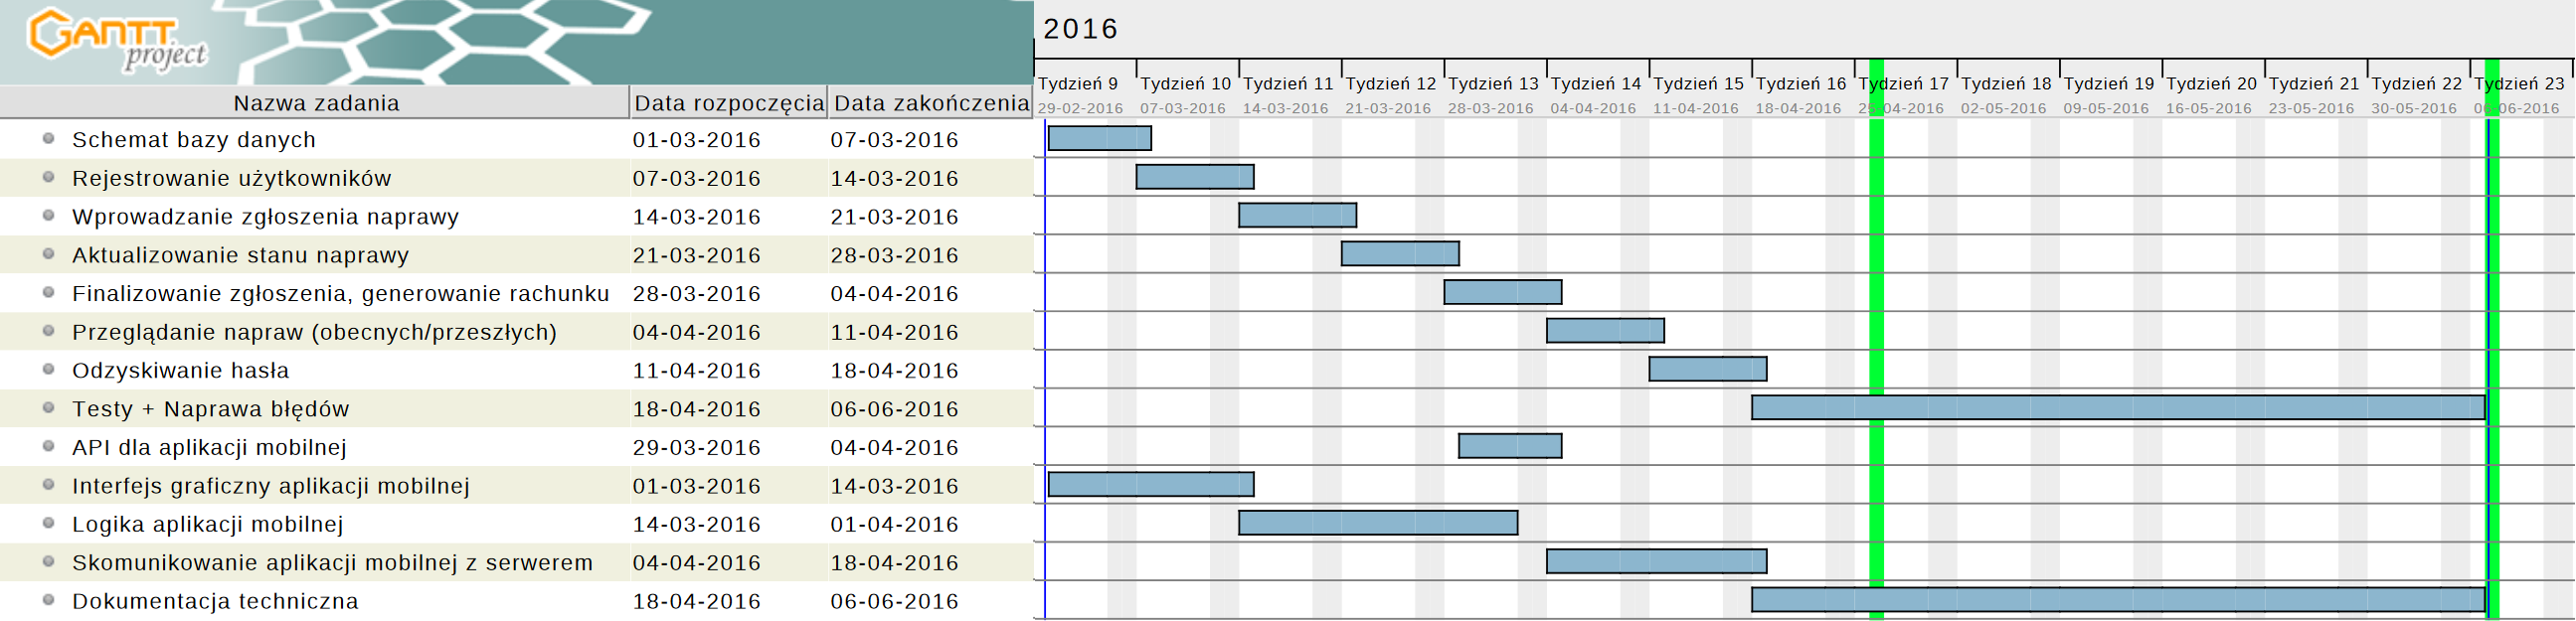
\includegraphics[width=1.3\textwidth,height=0.7\textheight]{gannth1.png}
	\caption{Wykres Gantta~- pierwszy kamień milowy}
\end{figure}
\end{landscape}
\begin{landscape}
Druga wersja diagramu Gantta powstała krótko przed osiągnięciem drugiego kamienia milowego. Został uzupełniony postęp poszczególnych funkcjonalności aplikacji, a~do listy zadań dodane zostały wybrane funkcjonalności rozszerzone. Poprawiony diagram znajduje się na rysunku 3.2.

\begin{figure}[h!]
	\centering
	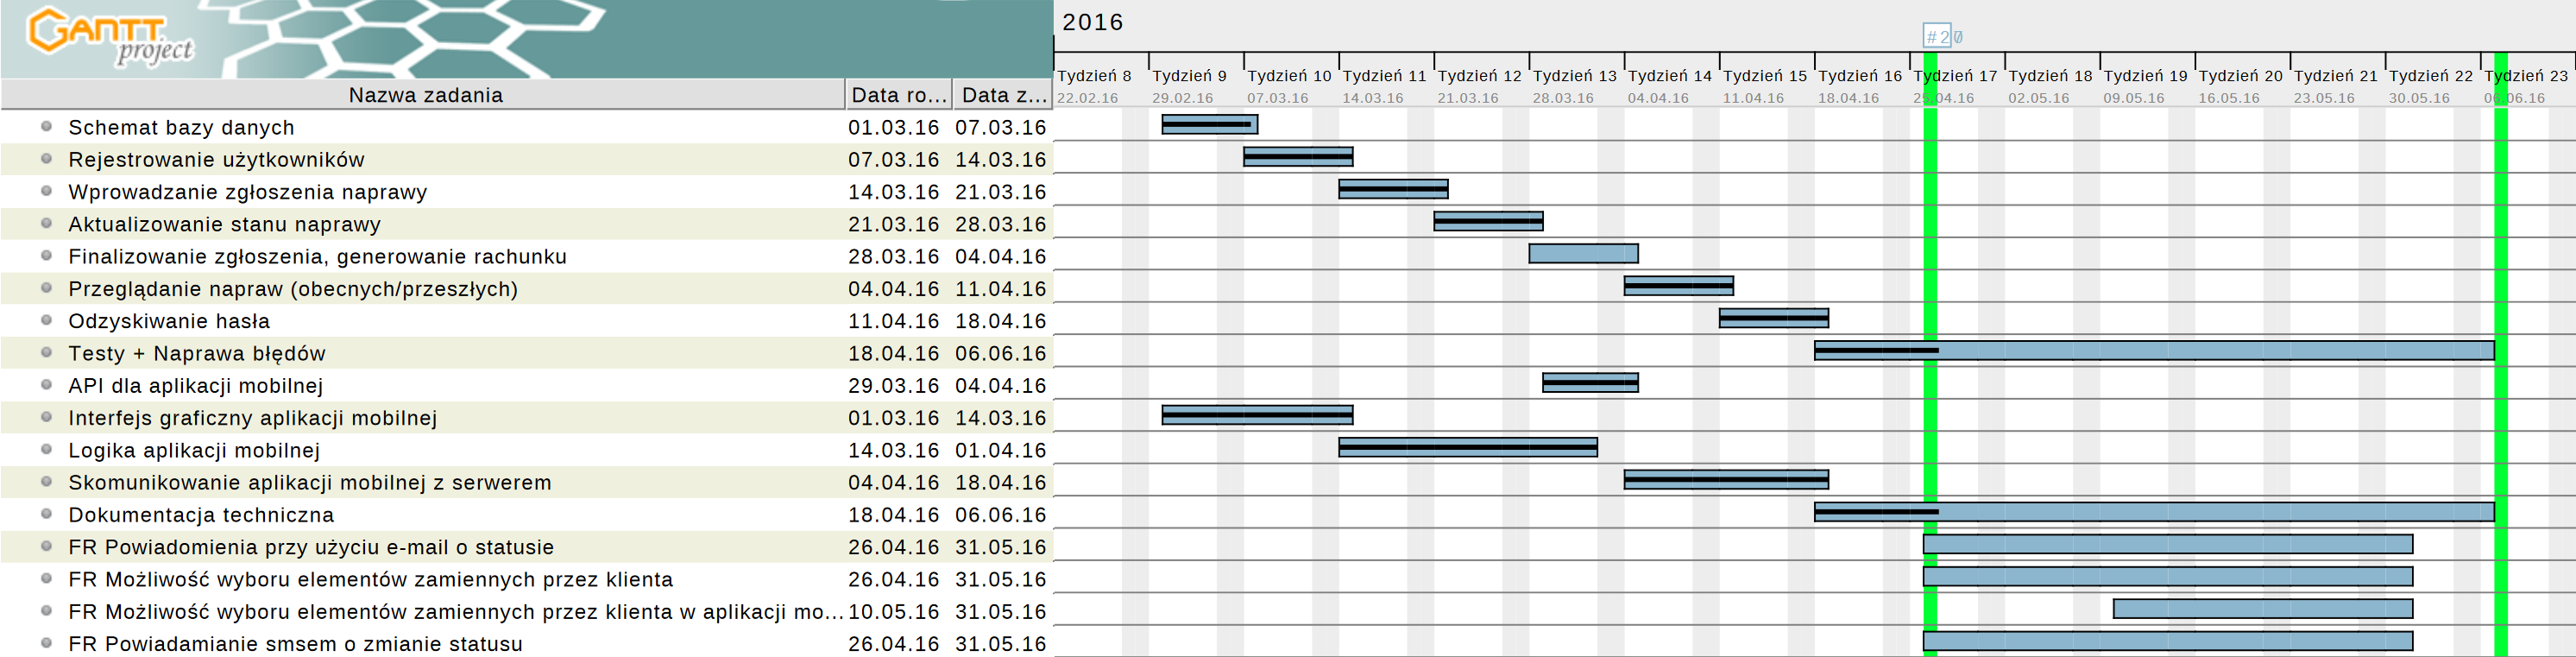
\includegraphics[width=1.3\textwidth,height=0.7\textheight]{gannth2.png}
	\caption{Wykres Gantta~- drugi kamień milowy}
\end{figure}
\end{landscape}
\begin{landscape}
Trzecia wersja diagramu Gantta powstała na sam koniec prac projektowych. Ponownie zaktualizowany został postęp poszczególnych funkcjonalności aplikacji, większość których została już ukończona w~100\%. Finalną wersję diagramu przedstawia rysunek 3.3.

\begin{figure}[h!]
	\centering
	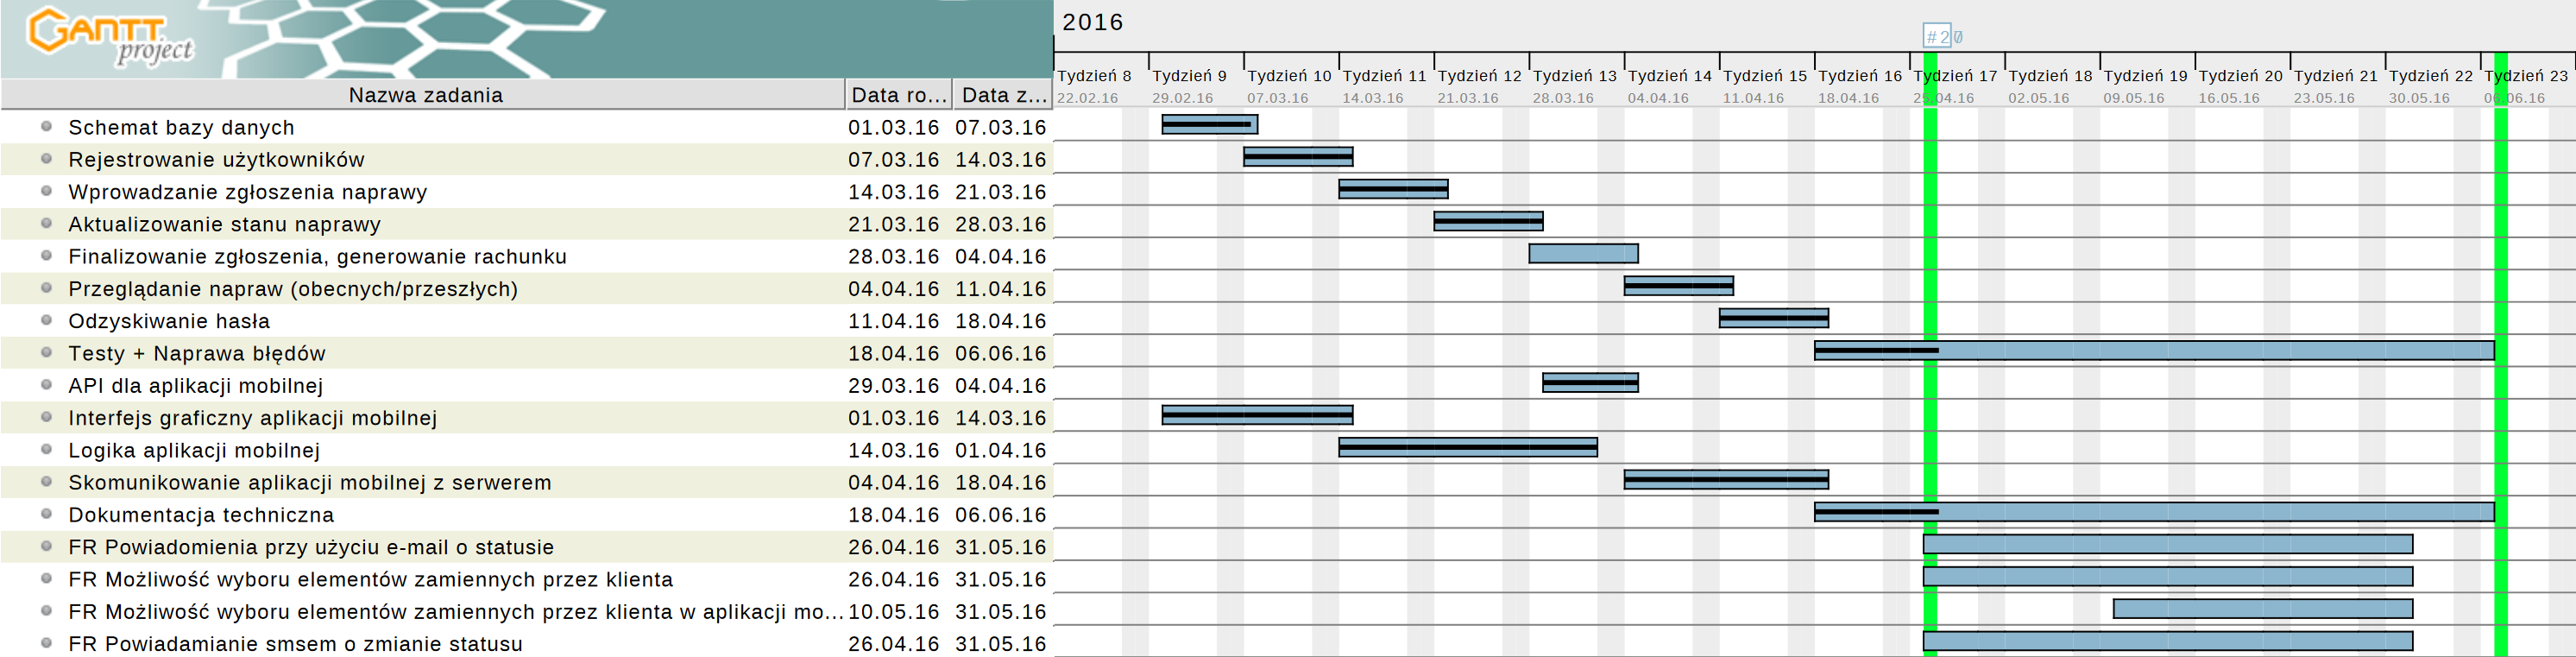
\includegraphics[width=1.3\textwidth,height=0.7\textheight]{gannth3.png}
	\caption{Wykres Gantta~- trzeci kamień milowy}
\end{figure}
\end{landscape}
\subsection{Rzeczywisty nakład pracy i~koszty}
Ze względu na otwarty charakter dostarczanego oprogramowania i~brak planowanych bezpośrednich zysków z~przedsięwzięcia zdecydowano o~nieokreśleniu średniej stawki godzinowej pracy członka zespołu w~projekcie. Konsekwentnie nie zostały obliczone sumaryczne koszty wytworzenia kompletnego produktu, jedynie nakład pracy wyrażony w~godzinach.
Rzeczywisty sumaryczny nakład pracy w~projekcie różni się od antycypowanego w~znaczącym stopniu ze względu na to, że podczas oryginalnego szacunku pominięto implementację funkcjonalności rozszerzonych aplikacji oraz stworzenie aplikacji mobilnej na urządzenia z~systemem Android. Pierwotny plan czasu pracy okazał się jednak być bardzo celny w~zakresie funkcjonalności podstawowych systemu. Rzeczywisty czas realizacji poszczególnych funkcjonalności  przedstawia tabela 3.2.
\begin{table}[H]
	\centering
	\caption{Faktyczny czas realizacji funkcjonalności}
	\bgroup
	\begin{tabular}{|l|c|c|}
		\hline
		\multicolumn{1}{|c|}{\textbf{Funkcjonalność}} & \textbf{Planowany czas} &\textbf{Rzeczywisty czas}\\ \hline \hline
		Stworzenie schematu bazy danych & 4h & 4h\\ \hline
		Rejestrowanie użytkowników w~systemie & 10h & 8h \\ \hline
		Wprowadzenie zgłoszenia naprawy & 11h & 9h \\ \hline
		Aktualizowanie stanu naprawy & 8h & 11h\\ \hline
		Finalizowanie zgłoszenia wraz z~generowaniem rachunku & 9h & 8h \\ \hline
		Przeglądanie napraw & 9h  & 8h\\ \hline
		Odzyskiwanie hasła & 5h & 5h\\ \hline
		Powiadomienie o~statusie przy użyciu e-mail & brak predykcji & 3h\\ \hline
		Powiadomienie o~statusie przy użyciu SMS & brak predykcji & niezrealizowane\\ \hline
		Wybór części zamiennych przez klienta & brak predykcji & 12h\\ \hline
		Implementacja aplikacji mobilnej & brak predykcji & 35h\\ \hline \hline
		\multicolumn{1}{|c|}{\textbf{Sumarycznie}} & \textbf{56h} & \textbf{103h} \\ \hline
	\end{tabular}
	\egroup
\end{table}


Sumaryczny przewidywany czas realizacji funkcjonalności wyniósł 56h, a~rzeczywisty czas realizacji funkcjonalności które zostały uwzględnione w~predykcjach był o~3 godziny krótszy (spadek o~5.4 \%). Sumaryczny czas wszystkich prac implementacyjnych wynosi 103h, co daje wzrost względem wartości planowanej o~83.9 \%, jednak należy powtórnie podkreślić że tak duża różnica wynika z~nieuwzględnienia prac nad aplikacją mobilną w~trakcie pierwotnych predykcji. Niezrealizowanie funkcjonalności służącej do powiadomienia użytkownika o~zmianie statusu zamówienia przez SMS wynikło z~nieprzewidzianych trudności realizacyjnych w~zakresie komunikacji pomiędzy serwerem a~bramką SMS~- problem na rozwiązanie którego trzeba by poświęcić więcej czasu niż ten jakim autorzy projektu dysponowali w~końcowej jego fazie.

\section{Implementacja i~wdrożenie projektu}
W ramach realizacji projektu zaimplementowana została wielowarstwowa aplikacja internetowa z~rozszerzeniem o~aplikację mobilną. Model bazy danych stworzono zgodnie z~podejściem „Database First” z~wykorzystaniem technologii ADO.NET. Jako narzędzie do mapowania obiektowo relacyjnego wykorzystano platformę Entity Framework, natomiast zapytania do bazy danych zostały napisane w~języku LINQ. Warstwa dostępu do danych została odseparowana od logiki aplikacji z~wykorzystaniem warstwy logiki biznesowej. Utworzone zostały modele transferu danych odzwierciedlające modele warstwy dostępu do danych oraz modele widoku je zawierające, po to aby uniknąć korzystania z~modeli warstwy dostępu do danych w~warstwie aplikacji.

Warstwa logiki aplikacji oraz warstwa prezentacji zostały zrealizowane w~oparciu o~platformę ASP.NET MVC 5. Autentykację użytkowników uzyskano z~wykorzystaniem ASP.NET Identity. Do tworzenia widoków aplikacji wykorzystano składnię Razor, a~sterowanie aplikacją zrealizowano za pomocą składnika platformy MVC o~nazwie HTML Helper; wykorzystano również składniki biblioteki jQuery UI. Od strony wizualnej widoki zostały zaprojektowane z~wykorzystaniem biblioteki Bootstrap oraz autorskich stylów CSS.

Dzięki ogromnym możliwościom dostarczonym przez Entity Framework pomimo relatywnie skomplikowanej struktury bazy danych operacje typu CRUD nie przysparzają żadnego problemu. Wielką zaletą stosowanego narzędzia jest fakt, że obiekty bazodanowe zawierają referencje do powiązanych ze sobą tabel, dzięki czemu w~bardzo prosty sposób można pobrać z~bazy dane z~powiązanych ze sobą tabel. Do mapowania obiektów warstwy dostępu do danych na obiekty transferowe wykorzystano Automapper. Podejście takie daje gwarancję że w~razie rozbudowy bazy danych wystarczy uzupełnić obiekty warstwy transferu danych o~nowe pola, nie trzeba natomiast przejmować się mapowaniem.

Aplikacja mobilna została napisana w~języku Android i~została zaprojektowana na urządzenia z~minimalną wersją systemu operacyjnego 4.0 (Ice Cream Sandwich). Aplikacja jest dostępna zarówno w~języku polskim jak i~angielskim. Do komunikacji z~serwerem wykorzystywane jest własnoręcznie stworzone API bazujące na metodach HTTP POST i~GET, a~dane są przesyłane w~formacie JSON. Aplikacja dzieli się na graficzny interfejs użytkownika (zawarty w~plikach xml) oraz część backendową (pliki java). Pierwszym widokiem otwieranym bezpośrednio po uruchomieniu aplikacji jest \texttt{activity\_login.xml}, a~klasy i~metody tej aktywności zostały zaimplementowane w~pliku LoginActivity.java. Wszystkie kolejne aktywności zostały zaimplementowane analogicznie jak w~powyższym przykładzie.

Wśród najważniejszych aktywności aplikacji mobilnej należy wyróżnić:
\begin{itemize}
	\item \texttt{activity\_login.xml}~- ekran logowania aplikacji  wyświetlający logo aplikacji i~pozwalający na zmianę języka,
	\item \texttt{activity\_panel\_components.xml}~- wyświetlenie dostępnej listy części zamiennych,
	\item \texttt{activity\_panel\_services.xml}~- wyświetlenie listy zgłoszeń użytkownika pokolorowanych w~zależności od ich statusu.
\end{itemize}
\subsection{Diagram technologii wykorzystanych w~projekcie}
Rysunek 4.1 przedstawia schemat połączeń pomiędzy poszczególnymi komponentami projektu i~wykorzystane technologie.
\begin{figure}[H]
	\centering
	\includegraphics[width=\textwidth,height=0.6\textheight]{diagramTechnologii.png}
	\caption{Diagram wykorzystanych technologii}
\end{figure}
\begin{landscape}
\subsection{Schemat bazy danych}
Rysunek 4.2 przedstawia schemat bazy danych zastosowanej w~projekcie.

\begin{figure}[h!]
	\centering
	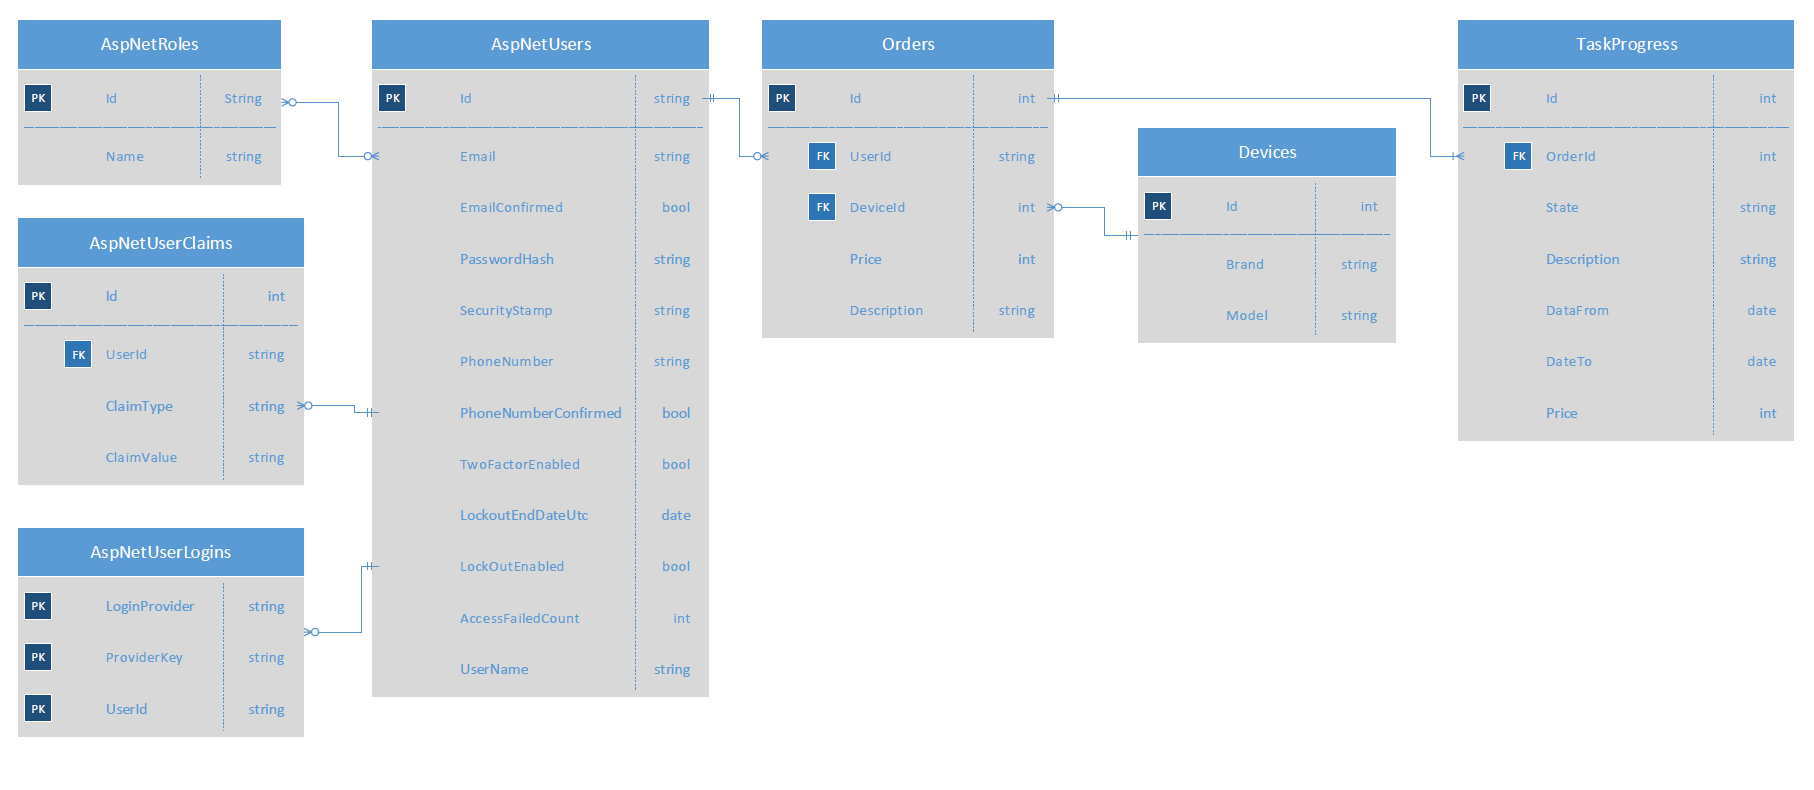
\includegraphics[width=1.3\textwidth,height=0.8\textheight]{dbSchema.png}
	\caption{Schemat bazy danych}
\end{figure}
\end{landscape}
\subsection{Instalacja projektu i~wymagania sprzętowe}
Ze względu na charakter projektu (open source) fizyczny proces wzdrożenia aplikacji we własnym serwisie napraw leży w~gestii właściciela serwisu. Jeśli posiada on własny serwer z~bazą danych MS SQL i~działającą usługą internetową IIS wystarczy wykonać następujące kroki:
\begin{itemize}
	\item folder zawierający stronę internetową umieścić w~folderze \texttt{C:\textbackslash inetpub\textbackslash wwwroot},
	\item przejść do \texttt{start -> uruchom -> inetmgr} aby otworzyć okno zarządzania aplikacjami internetowymi i~uruchomić serwer (patrz rysunek 4.3).
\end{itemize}
\begin{figure}[h!]
	\centering
	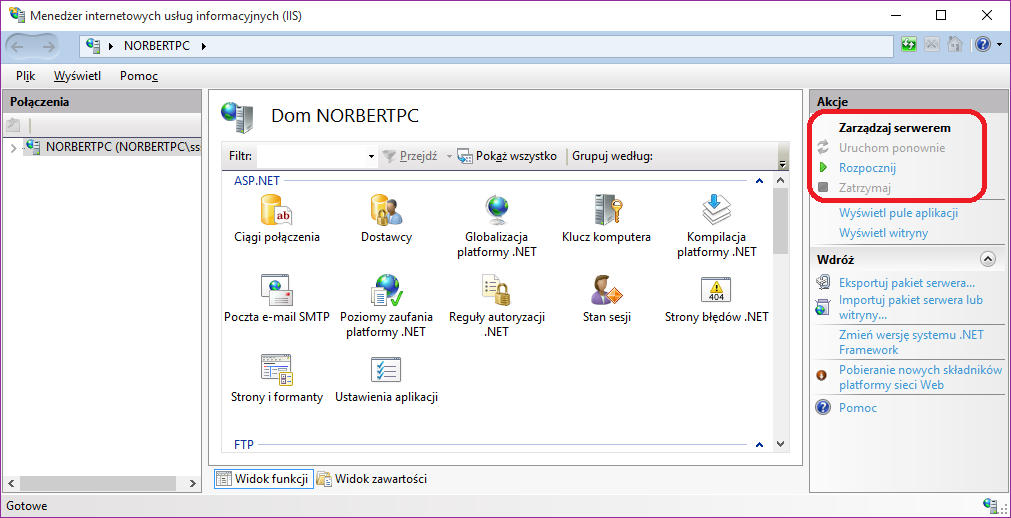
\includegraphics[width=\textwidth,height=0.6\textheight]{inetMgr.png}
	\caption{Ręczne uruchomienie serwera na lokalnej maszynie}
\end{figure}
Jeśli jednak użytkownik nie posiada takiej możliwości zachodzi konieczność wykupienia hostingu. Przykładowym portalem oferującym zarówno serwer usług internetowych IIS jak i~serwer bazodanowy MS SQL jest witryna somee.com. Po ukończeniu procesu rejestracji i~wykupieniu żądanego przez nas planu usługowego możemy utworzyć swoją stronę internetową, co zostało przedstawione na rysunkach 4.4 i~4.5.
\begin{figure}[H]
	\centering
	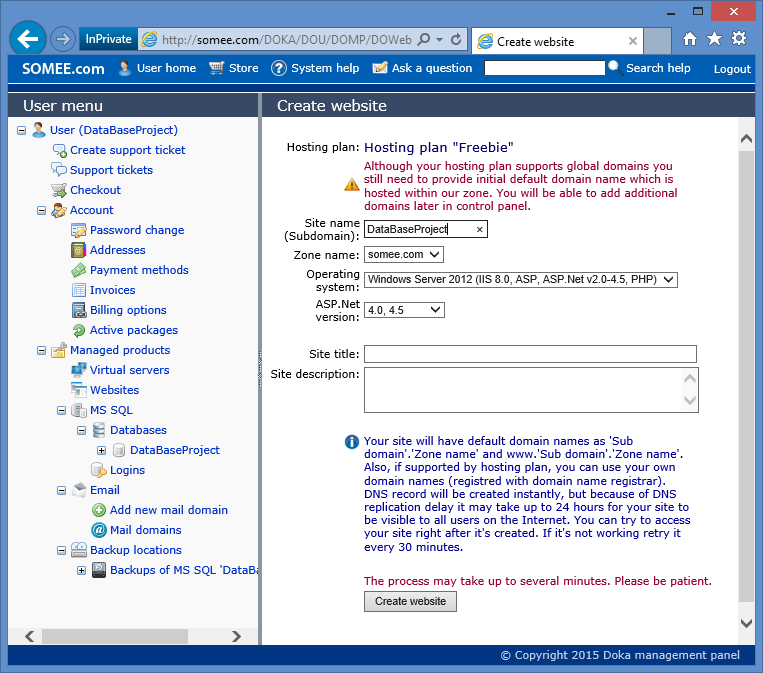
\includegraphics[width=\textwidth,height=0.6\textheight]{somee1.png}
	\caption{Zakładanie strony internetowej cz.1}
\end{figure}
\begin{figure}[H]
	\centering
	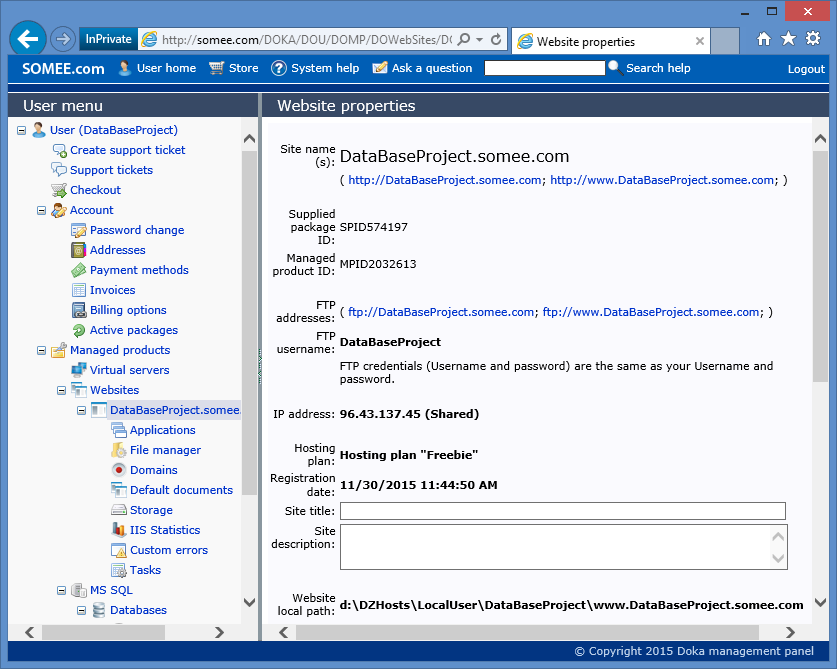
\includegraphics[width=\textwidth,height=0.6\textheight]{somee2.png}
	\caption{Zakładanie strony internetowej cz.2}
\end{figure}
Następnym krokiem jest instalacja naszej aplikacji na zdalnym serwerze. Proces ten znacząco może uprościć IDE Visual Studio, wymagając od użytkownika jedynie kliknięcia opcji \texttt{publish} i~wybrania profilu publikacji. Przedstawiają to rysunki 4.6 i~4.7.
\begin{figure}[H]
	\centering
	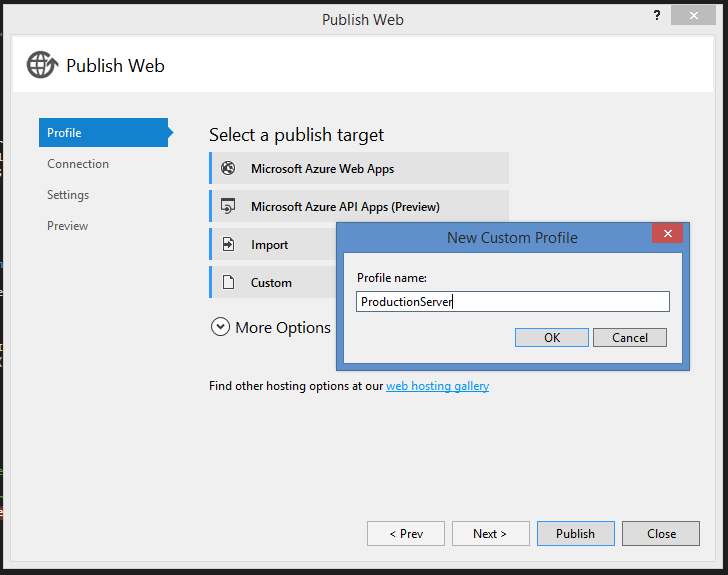
\includegraphics[width=\textwidth,height=0.4\textheight]{vs2.png}
	\caption{Tworzenie profilu}
\end{figure}
\begin{figure}[H]
	\centering
	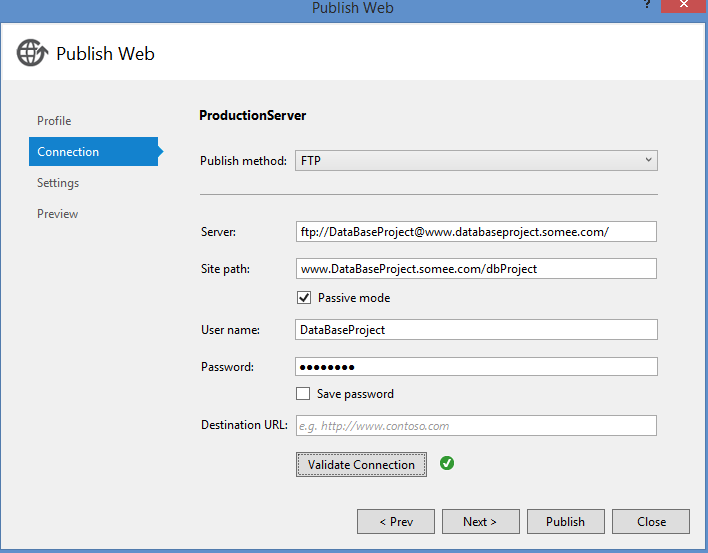
\includegraphics[width=\textwidth,height=0.4\textheight]{vs3.png}
	\caption{Wybór adresu serwera i~publikacja projektu}
\end{figure}
Ostatnim brakującym elementem układanki jest połączenie serwera z~bazą danych. Analogicznie jak w~przypadku samej aplikacji, jeśli nie mamy możliwości umieszczenia jej na własnym serwerze jesteśmy zmuszeni skorzystać z~hostingu wykonując proces zbliżony do publikowania samej aplikacji. Dodatkowo aby zapewnić komunikację pomiędzy aplikacją a~bazą danych należy zdefiniować odpowiedni connection string w~pliku konfiguracyjnym Web.config. Czynności te zostały zaprezentowane na rysunkach od 4.8 do 4.10.
\begin{figure}[H]
	\centering
	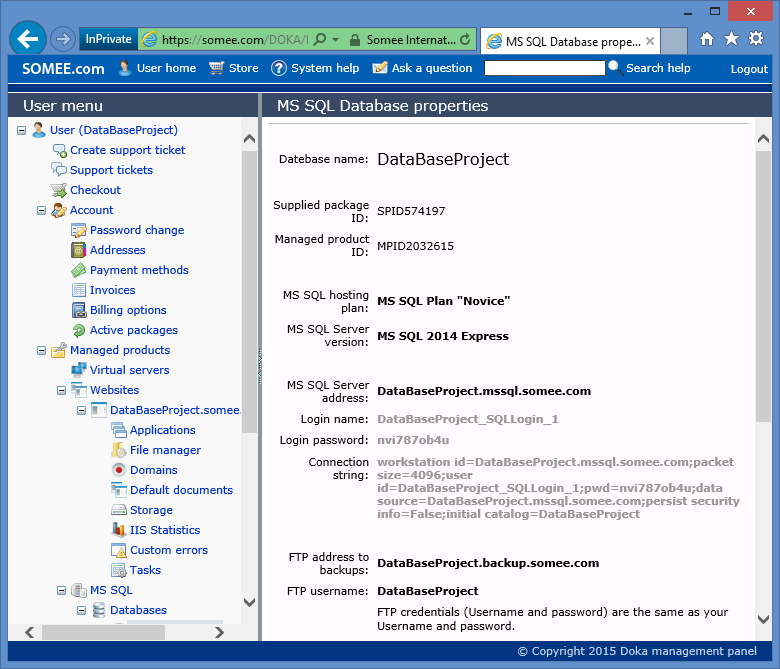
\includegraphics[width=\textwidth,height=0.6\textheight]{db1.png}
	\caption{Hosting bazy danych}
\end{figure}
\begin{figure}[H]
	\centering
	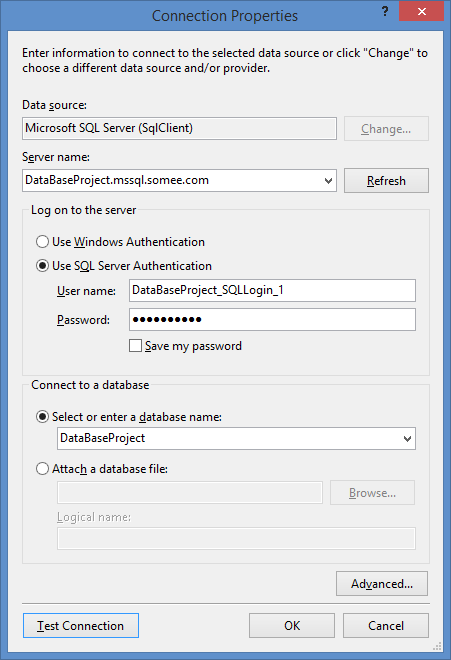
\includegraphics[width=0.6\textwidth,height=0.42\textheight]{db3.png}
	\caption{Ustawienia połączenia}
\end{figure}
\begin{figure}[h!]
	\centering
	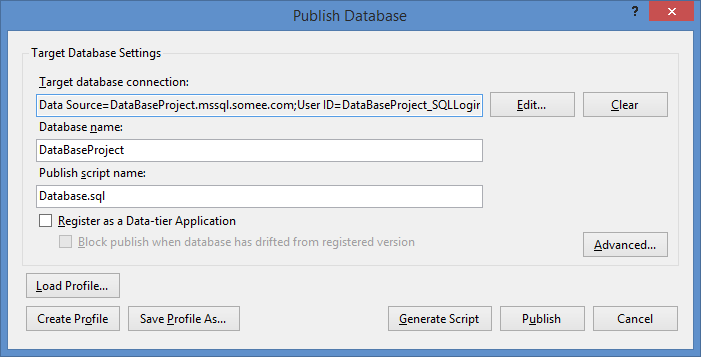
\includegraphics[width=\textwidth,height=0.4\textheight]{db4.png}
	\caption{Publikacja bazy danych}
\end{figure}

Wdrożenie aplikacji mobilnej jest relatywnie prostym procesem. Po umieszczeniu aplikacji webowej na wybranym serwerze należy zmienić wykorzystywany URL w~czterech plikach źródłowych aplikacji (\texttt{services\_details.java, panel\_services.java, panel\_components.java i~LoginActivity.java}) na adres działającego własnego serwera, a~następnie zbudować całą aplikację od początku. Otrzymany plik \texttt{*.apk} możemy już udostępnić do pobrania klientom serwisu np. poprzez istniejącą stronę internetową.
\subsection{Prezentacja działania i~instrukcja obsługi systemu}
\subsubsection{Aplikacja webowa}
W ramach testowania realizowanego projektu serwer aplikacji i~bazodanowy zostały umieszczone w~chmurze Azure udostępnianej przez firmę Microsoft. Po otwarciu strony
\begin{center}
	\vspace{-0.2cm}
	\texttt{http://serviceofelectronicdevices.azurewebsites.net/}
\end{center} 
\vspace{-0.2cm} pokazuje się ekran powitalny przedstawiony na rysunku 4.11.

\begin{figure}[H]
	\centering
	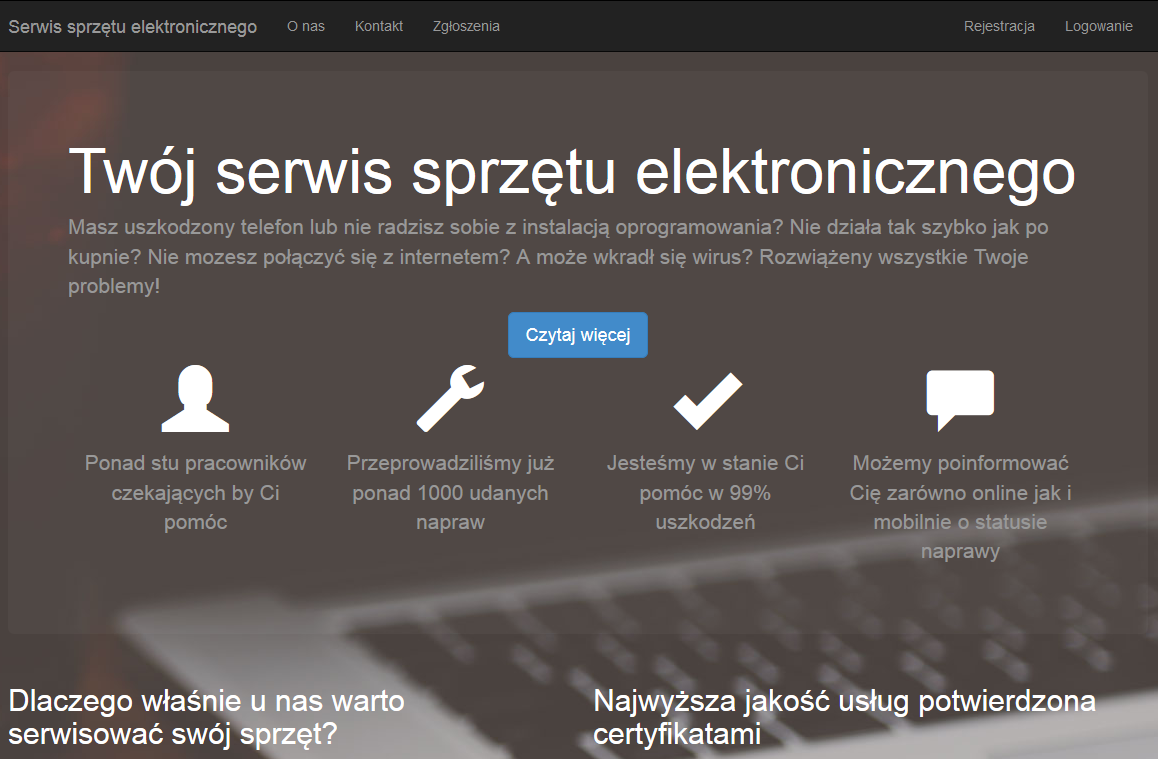
\includegraphics[width=\textwidth,height=0.55\textheight]{serwisGlowna.png}
	\caption{Strona główna serwisu}
\end{figure}

Rysunek 4.12 przedstawia informacje o~stronie internetowej, 4.13 formularz rejestracji nowego użytkownika a~4.14 panel logowania.
\begin{figure}[H]
	\centering
	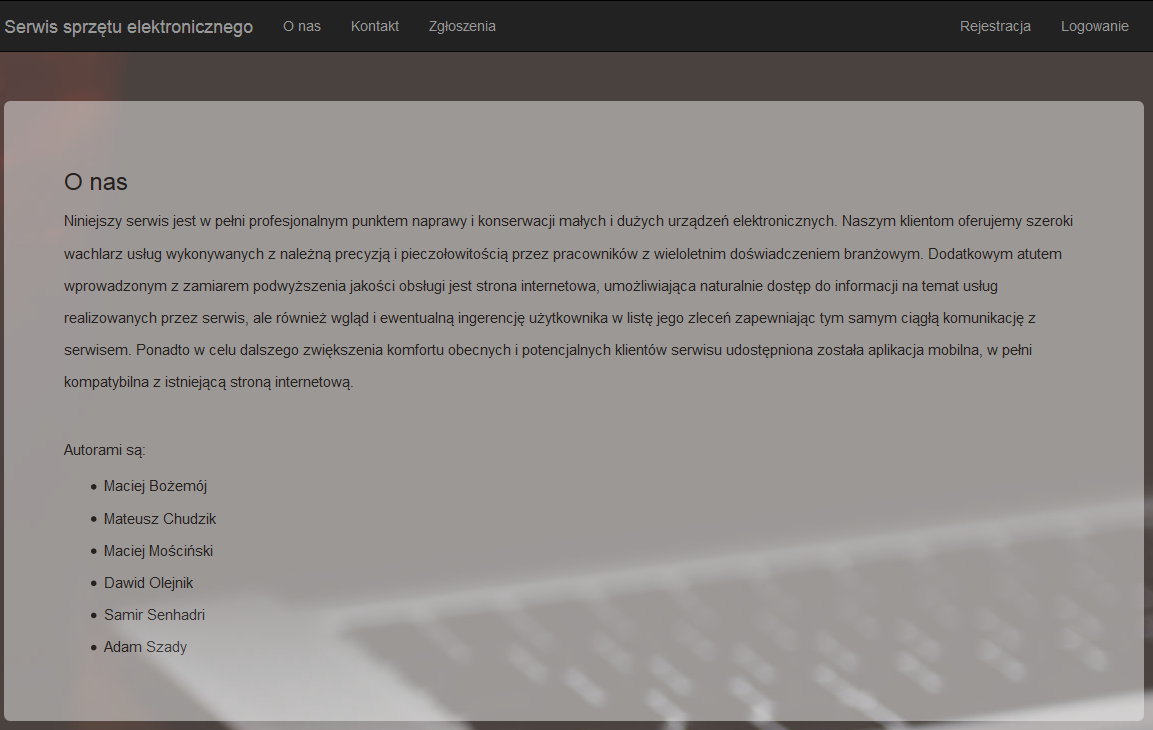
\includegraphics[width=\textwidth,height=0.6\textheight]{serwisOnas.png}
	\caption{Informacje o~serwisie}
\end{figure}
\begin{figure}[H]
	\centering
	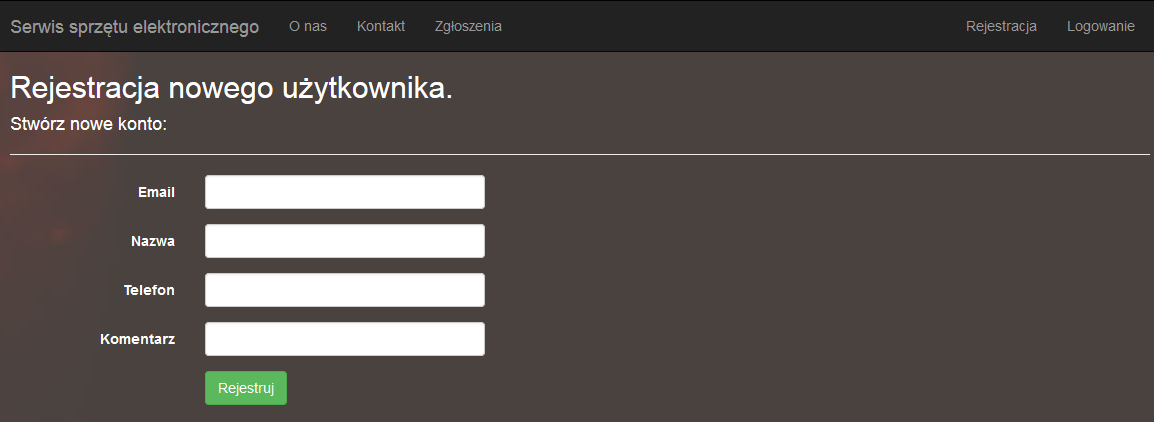
\includegraphics[width=\textwidth,height=0.32\textheight]{serwisRejestracja.png}
	\caption{Formularz rejestracji}
\end{figure}
\begin{figure}[H]
	\centering
	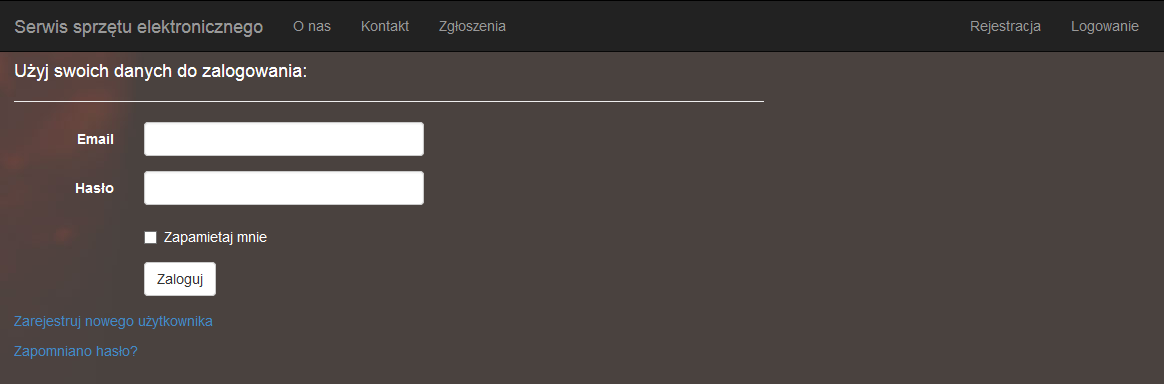
\includegraphics[width=\textwidth,height=0.3\textheight]{serwisLogowanie.png}
	\caption{Panel logowania}
\end{figure}

Po zalogowaniu mamy dostęp do listy zleceń oraz, zależnie od uprawnień użytkownika, innych funkcjonalności systemu. Wyróżniamy trzy różne poziomy uprawnień użytkowników~- klient, pracownik i~administrator systemu. Rysunki od 4.15 do 4.17 przedstawiają widok zleceń dla kolejno wzrastających poziomów uprawnień.

\begin{figure}[H]
	\centering
	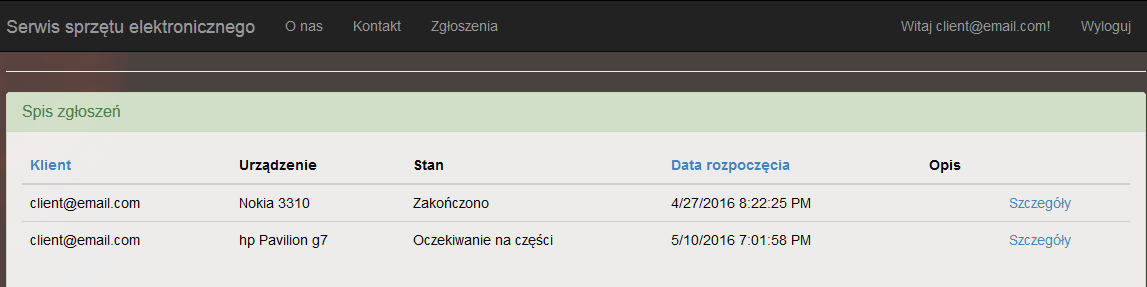
\includegraphics[width=\textwidth,height=0.2\textheight]{serwisKlient.png}
	\caption{Zlecenia~- klient}
\end{figure}
\begin{figure}[H]
	\centering
	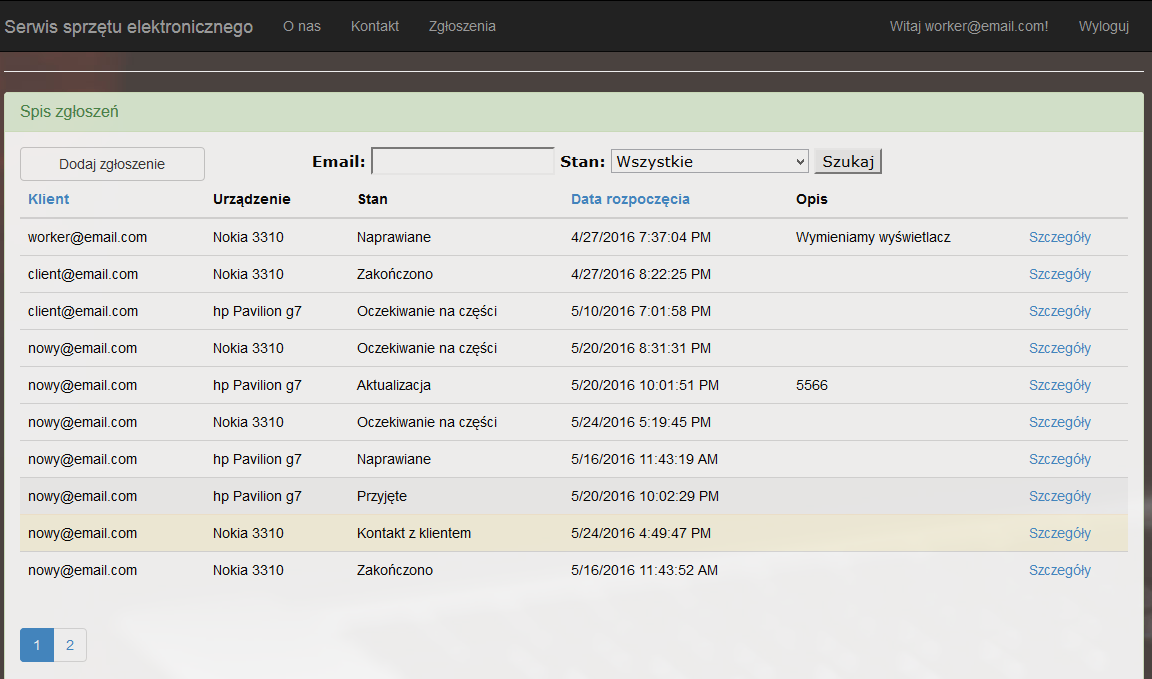
\includegraphics[width=\textwidth,height=0.6\textheight]{serwisWorker.png}
	\caption{Zlecenia~- pracownik}
\end{figure}
\begin{figure}[H]
	\centering
	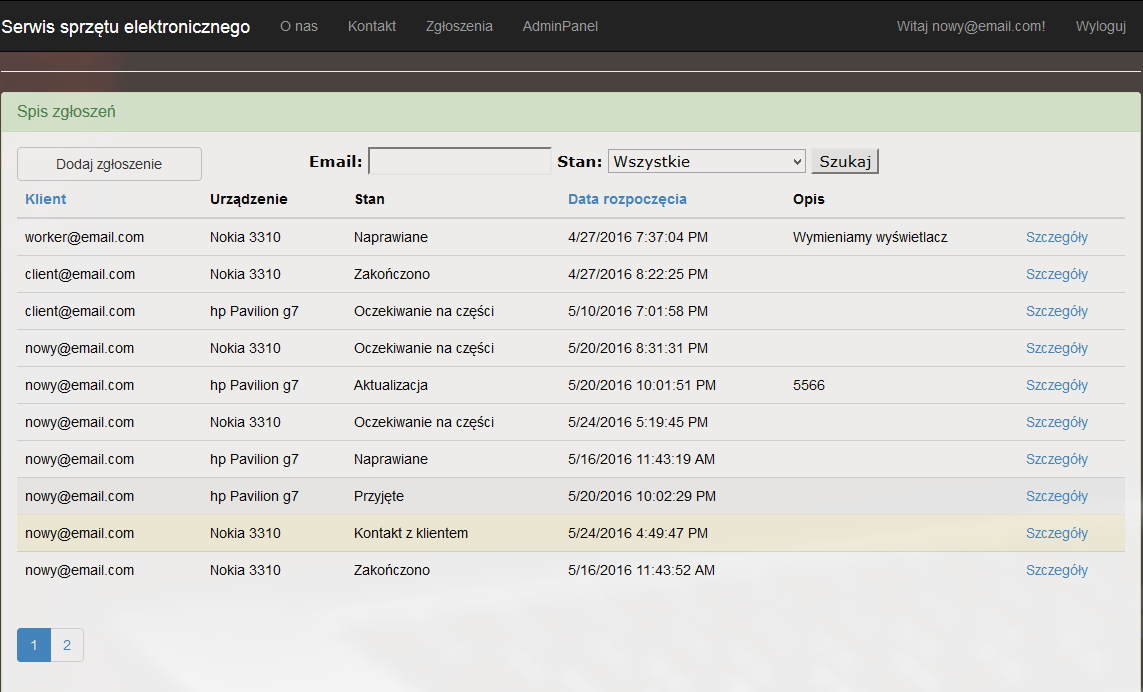
\includegraphics[width=\textwidth,height=0.6\textheight]{serwisZlecenia.png}
	\caption{Zlecenia~- administrator}
\end{figure}
\newpage
Administrator systemu dodatkowo ma dostęp do panelu administracyjnego, z~którego może dodawać i~odbierać role innym użytkownikom oraz zarządzać częściami i~produktami wykorzystywanymi w~serwisie. Przedstawia to rysunek 4.18.

\begin{figure}[H]
	\centering
	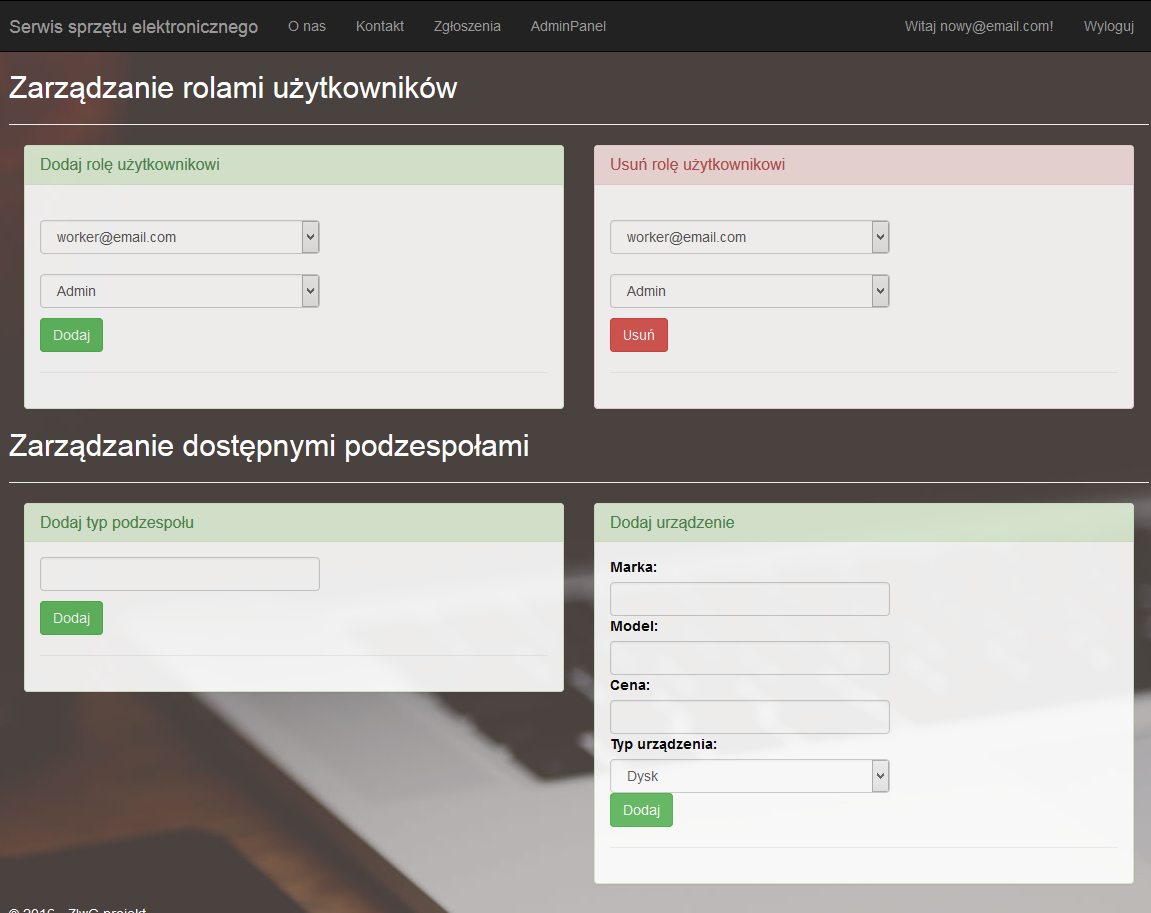
\includegraphics[width=\textwidth,height=0.6\textheight]{serwisAdmin.png}
	\caption{Panel administracyjny}
\end{figure}
\newpage
Wszyscy użytkownicy systemu mają możliwość podejrzenia szczegółów zamówienia - ekran ten przedstawia rysunek 4.19.
\begin{figure}[H]
	\centering
	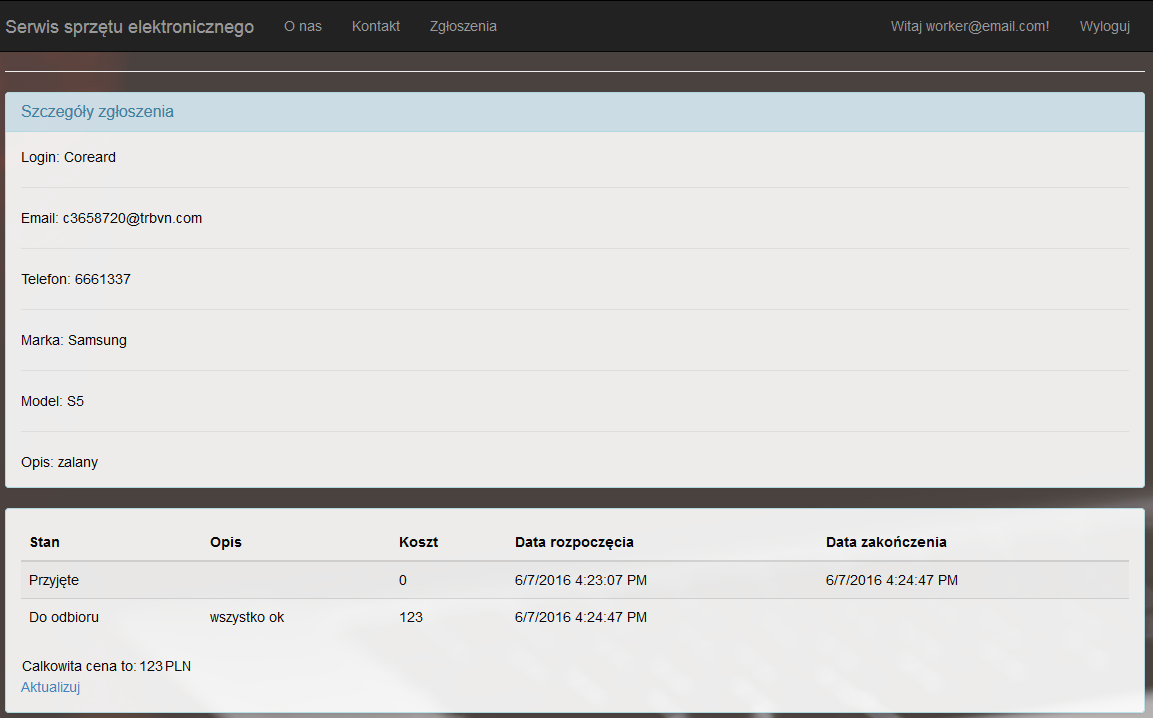
\includegraphics[width=\textwidth,height=0.6\textheight]{szczegoly.png}
	\caption{Szczegóły zamówienia}
\end{figure}
Użytkownicy o poziomie dostępu co najmniej pracownika mogą edytować szczegóły zamówienia (patrz rysunek 4.20).
\begin{figure}[H]
	\centering
	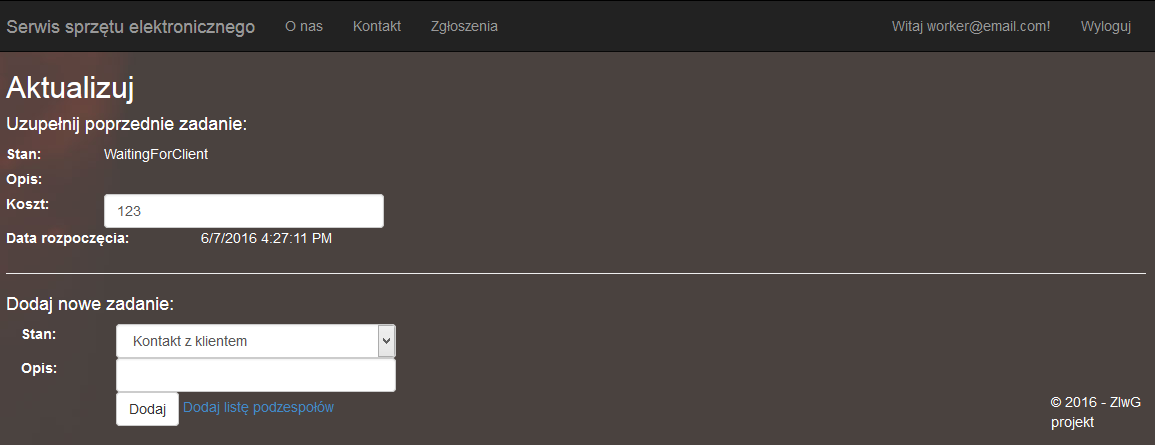
\includegraphics[width=\textwidth,height=0.3\textheight]{aktualizacja.png}
	\caption{Aktualizacja zamówienia}
\end{figure}
Na rysunku 4.21 została przedstawiona historia zmian danej naprawy i możliwość wyboru części przez klienta.
\begin{figure}[H]
	\centering
	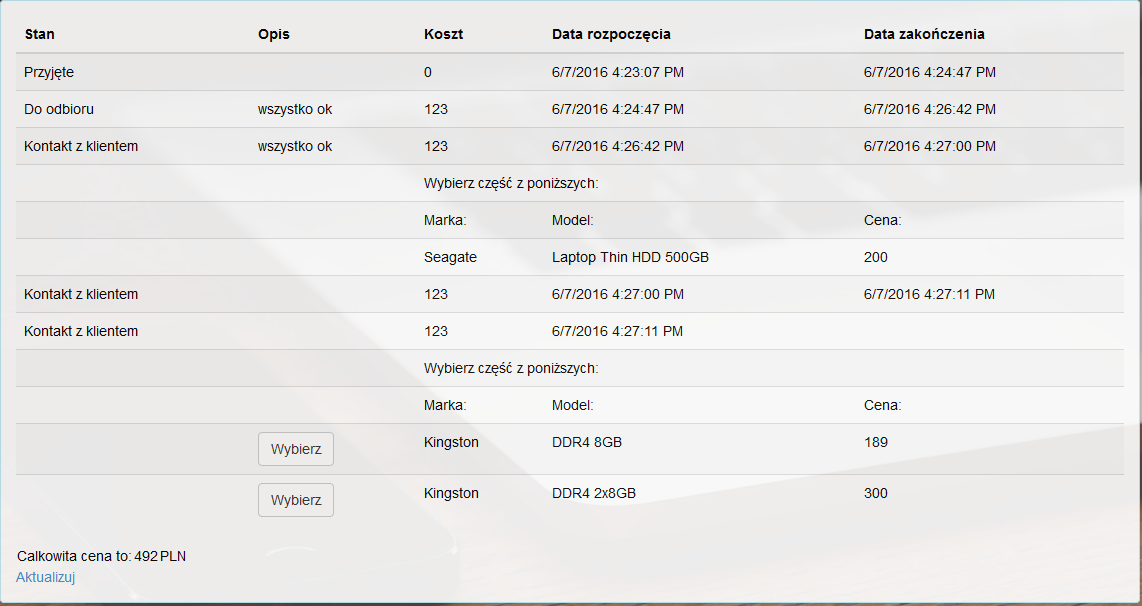
\includegraphics[width=\textwidth,height=0.5\textheight]{historia.png}
	\caption{Historia zmian i wybór części}
\end{figure}
\subsubsection{Aplikacja mobilna}
Jako że aplikacja mobilna zawiera w~sobie tylko część funkcjonalności aplikacji webowej jej obsługa jest tym bardziej prosta i~intuicyjna. Działanie aplikacji zostanie przedstawione z~wykorzystaniem jej polskiej wersji językowej. Rysunki od 4.22 do 4.26 przedstawiają kolejno:
\begin{itemize}
	\item ekran logowania aplikacji,
	\item ekran powitalny po zalogowaniu,
	\item profil zalogowanego użytkownika,
	\item podgląd zleceń użytkownika,
	\item podgląd szczegółów zlecenia.
\end{itemize}

\begin{figure}[H]
	\centering
	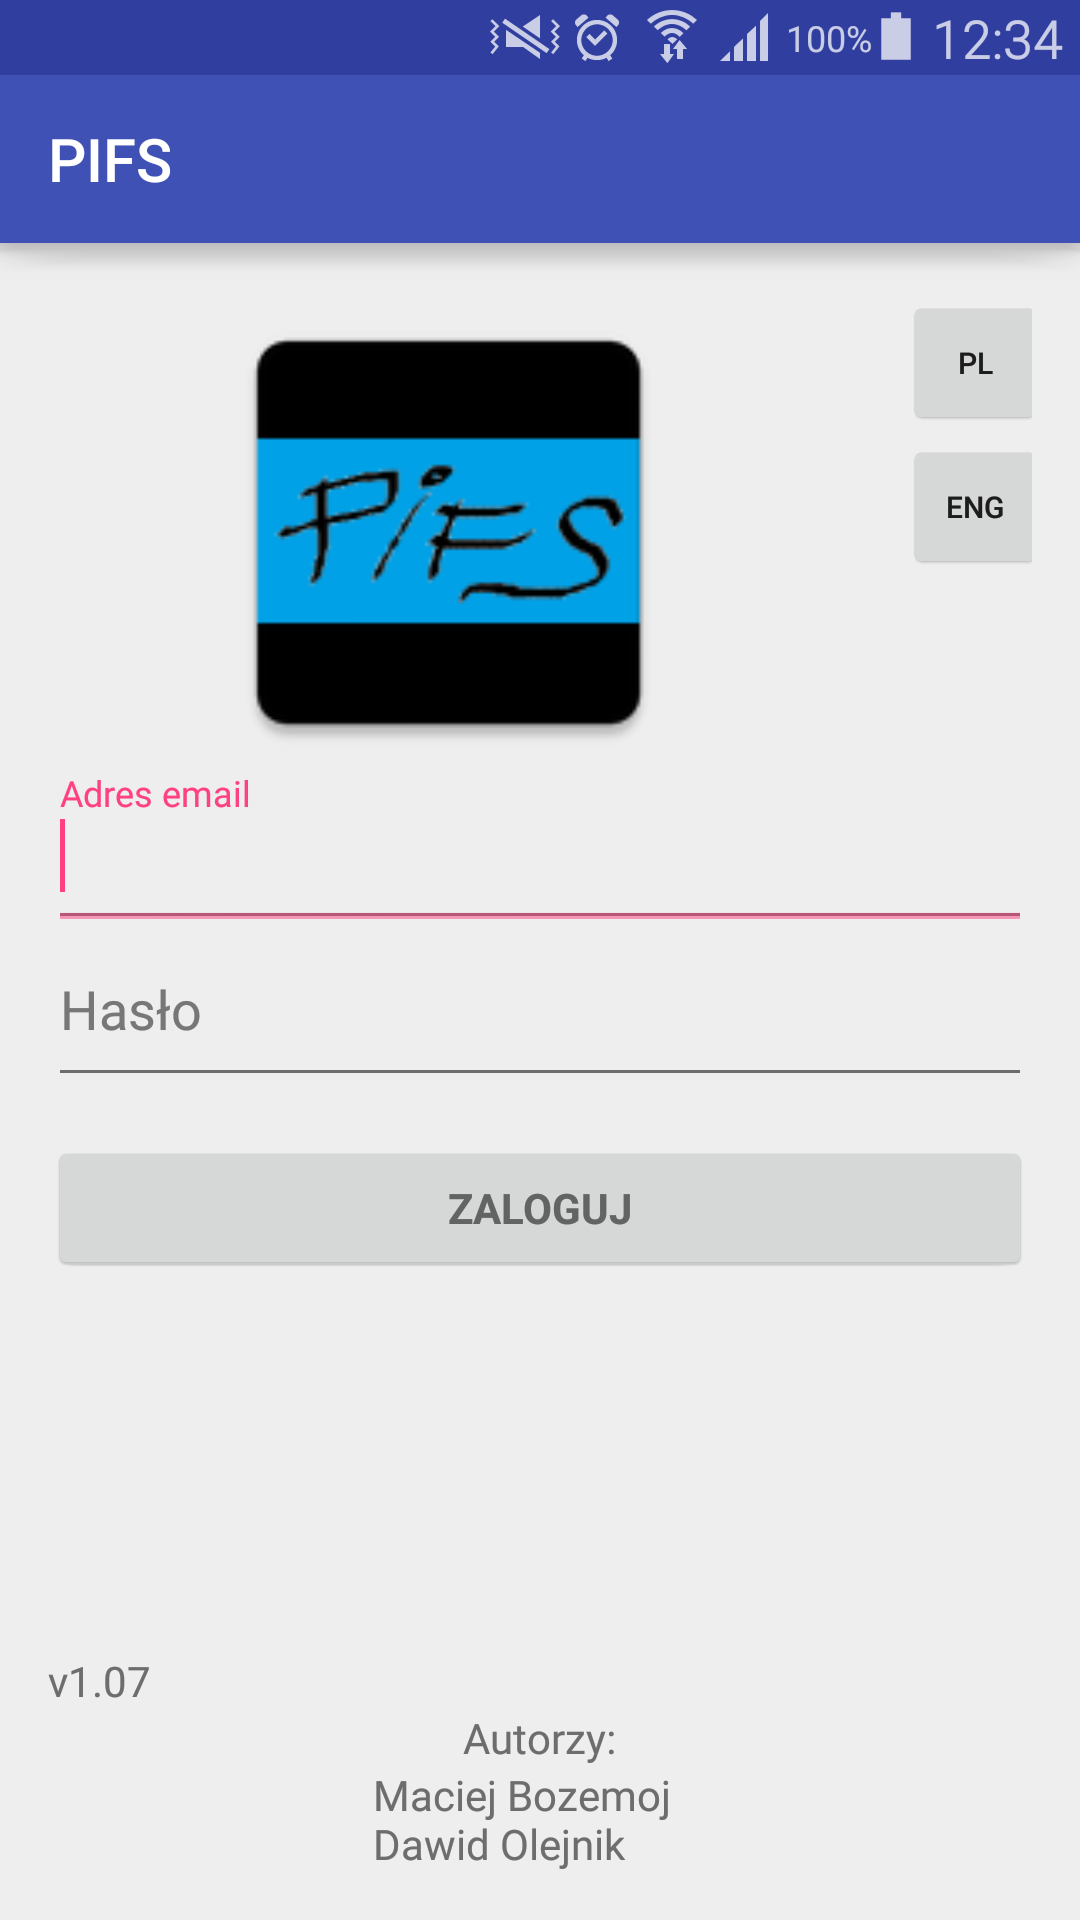
\includegraphics[width=0.6\textwidth,height=0.9\textheight]{startPolski.png}
	\caption{Logowanie}
\end{figure}


\begin{figure}[H]
	\centering
	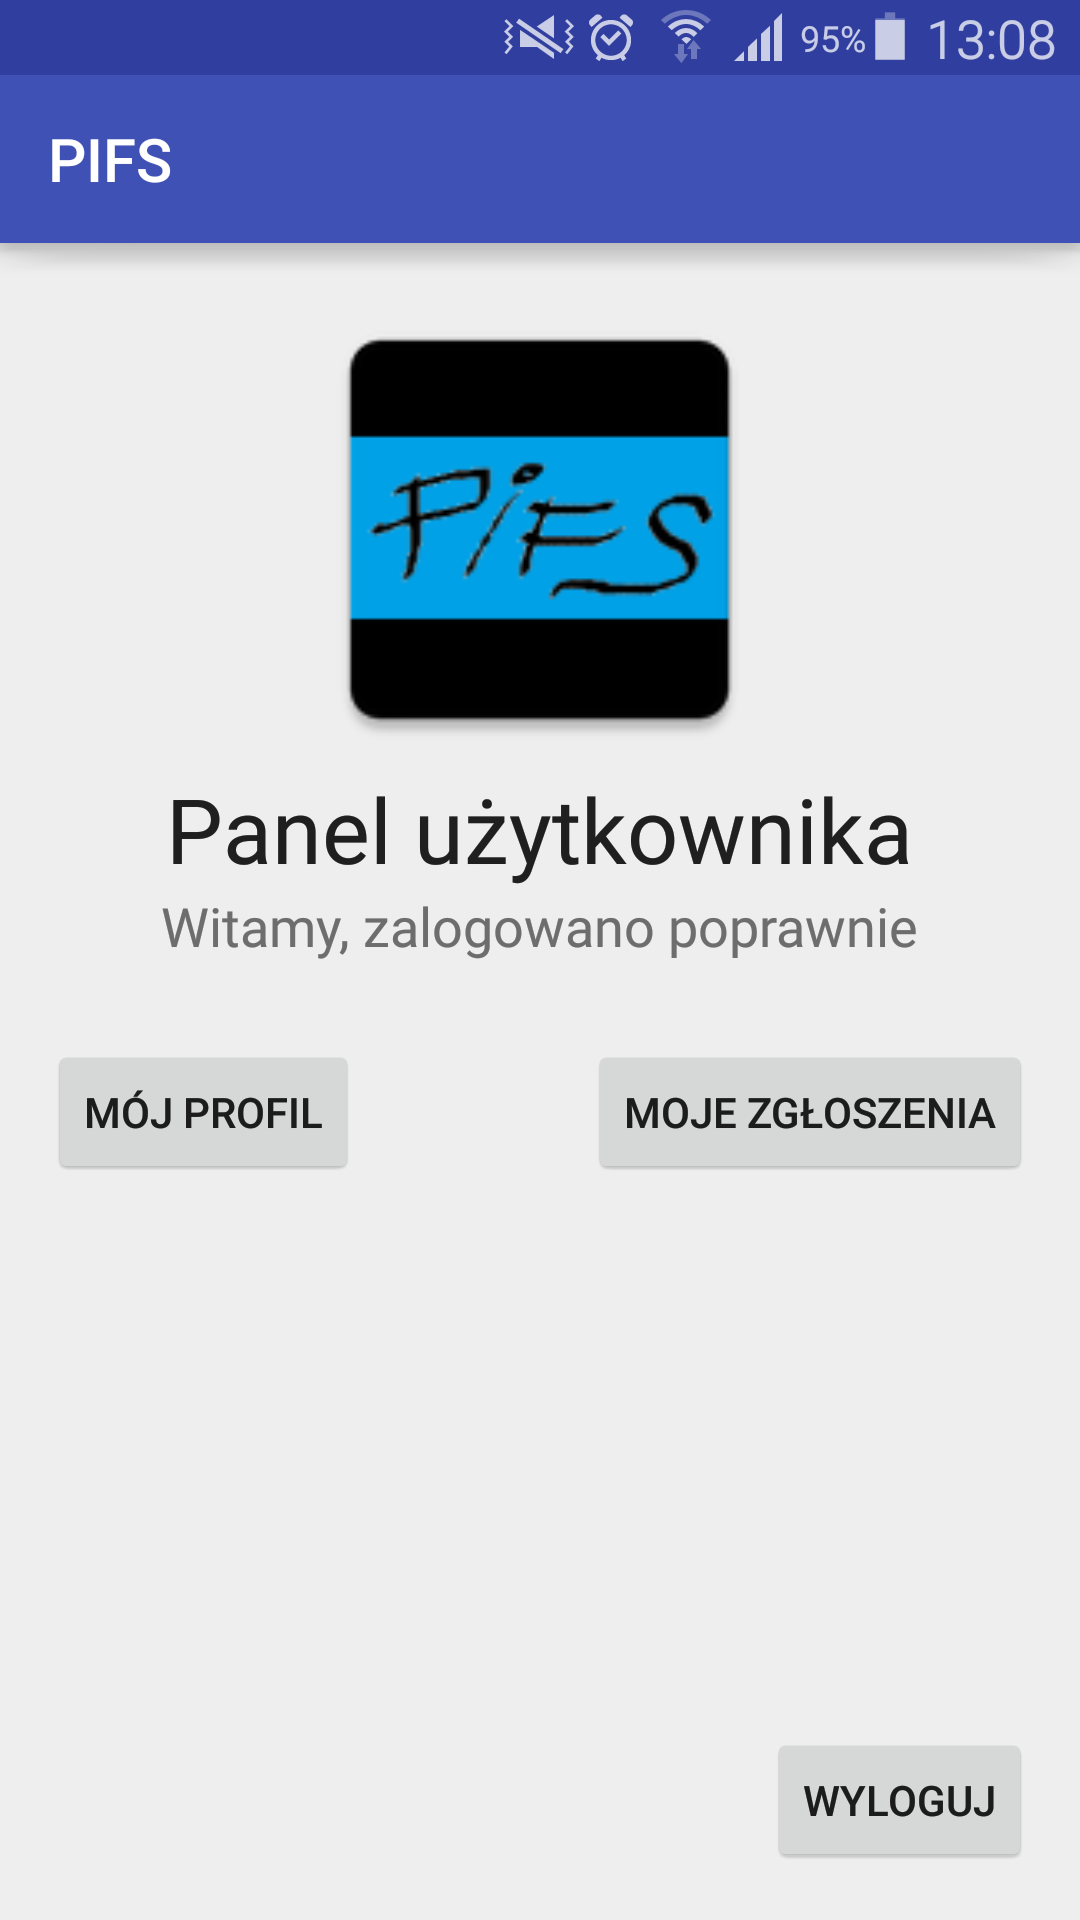
\includegraphics[width=0.6\textwidth,height=0.9\textheight]{logowaniePolski.png}
	\caption{Ekran powitalny}
\end{figure}


\begin{figure}[H]
	\centering
	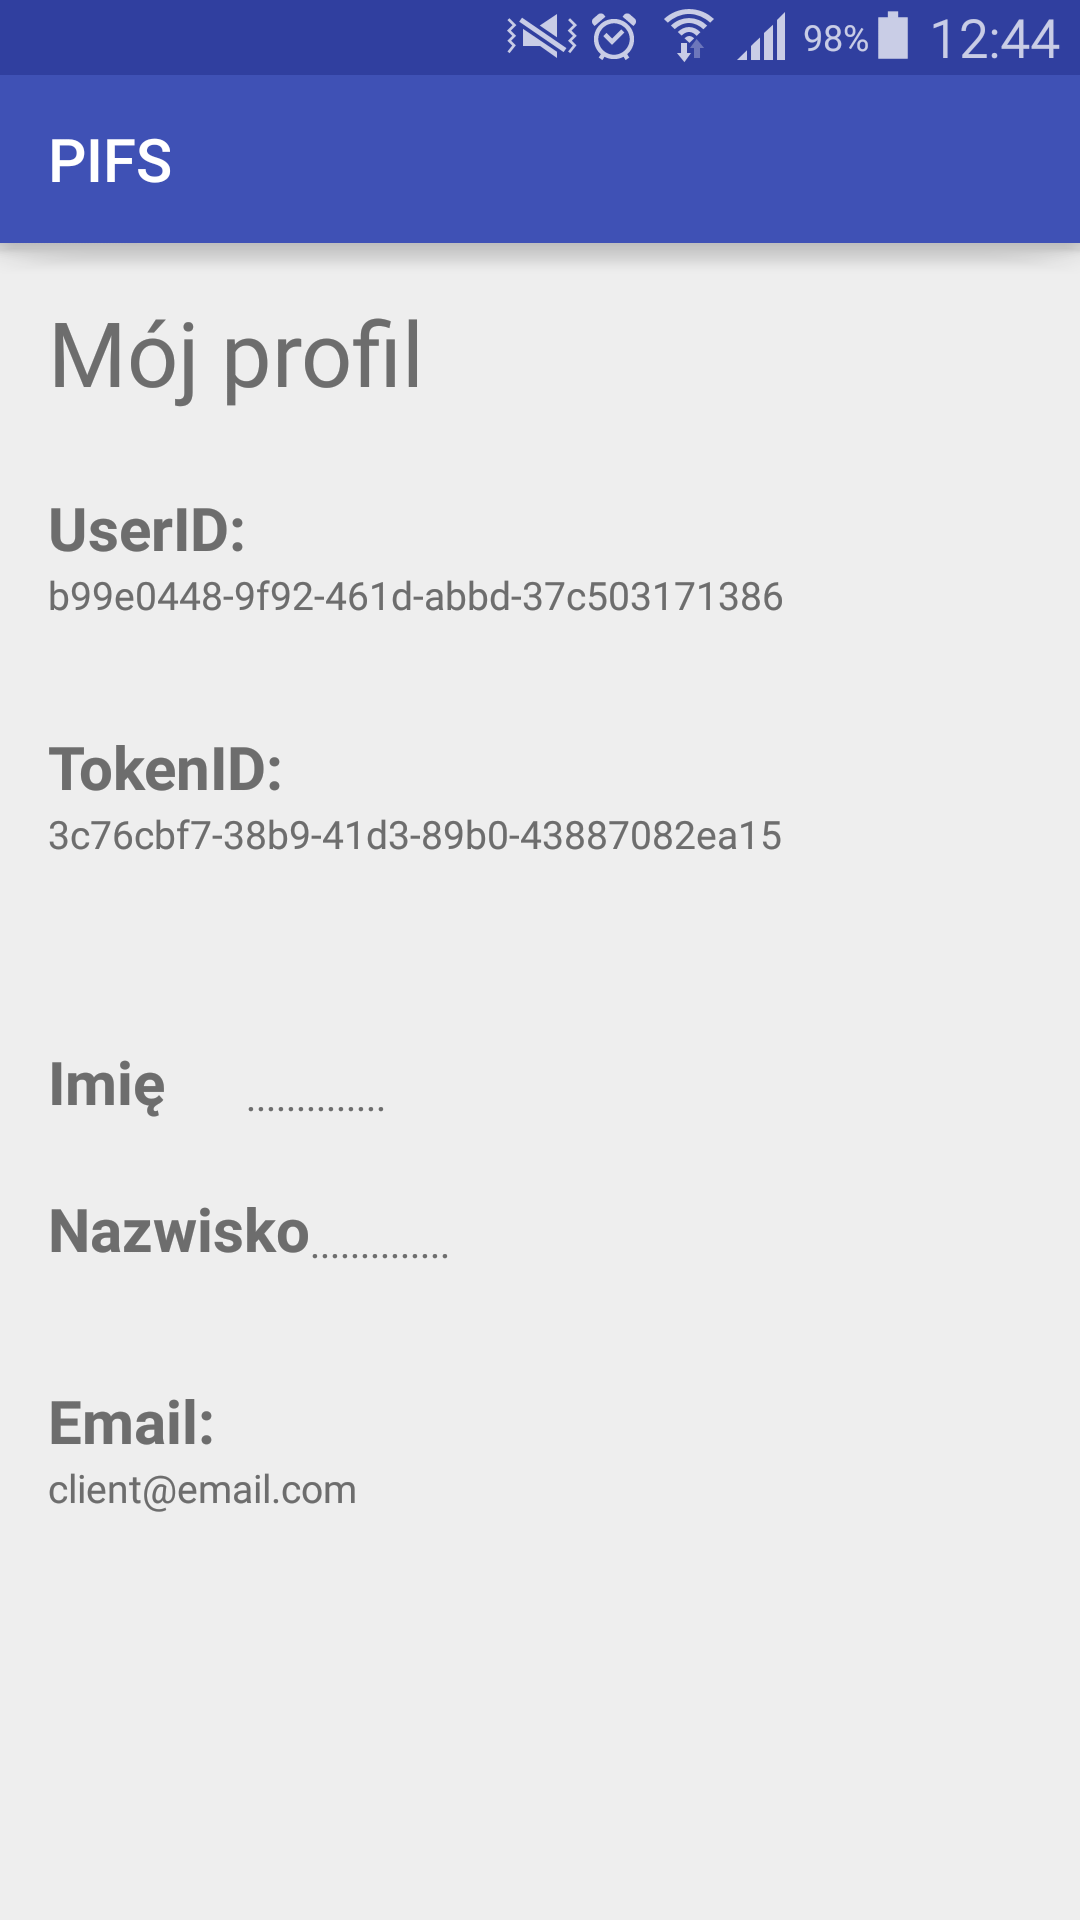
\includegraphics[width=0.6\textwidth,height=0.9\textheight]{profilPolski.png}
	\caption{Profil użytkownika}
\end{figure}


\begin{figure}[H]
	\centering
	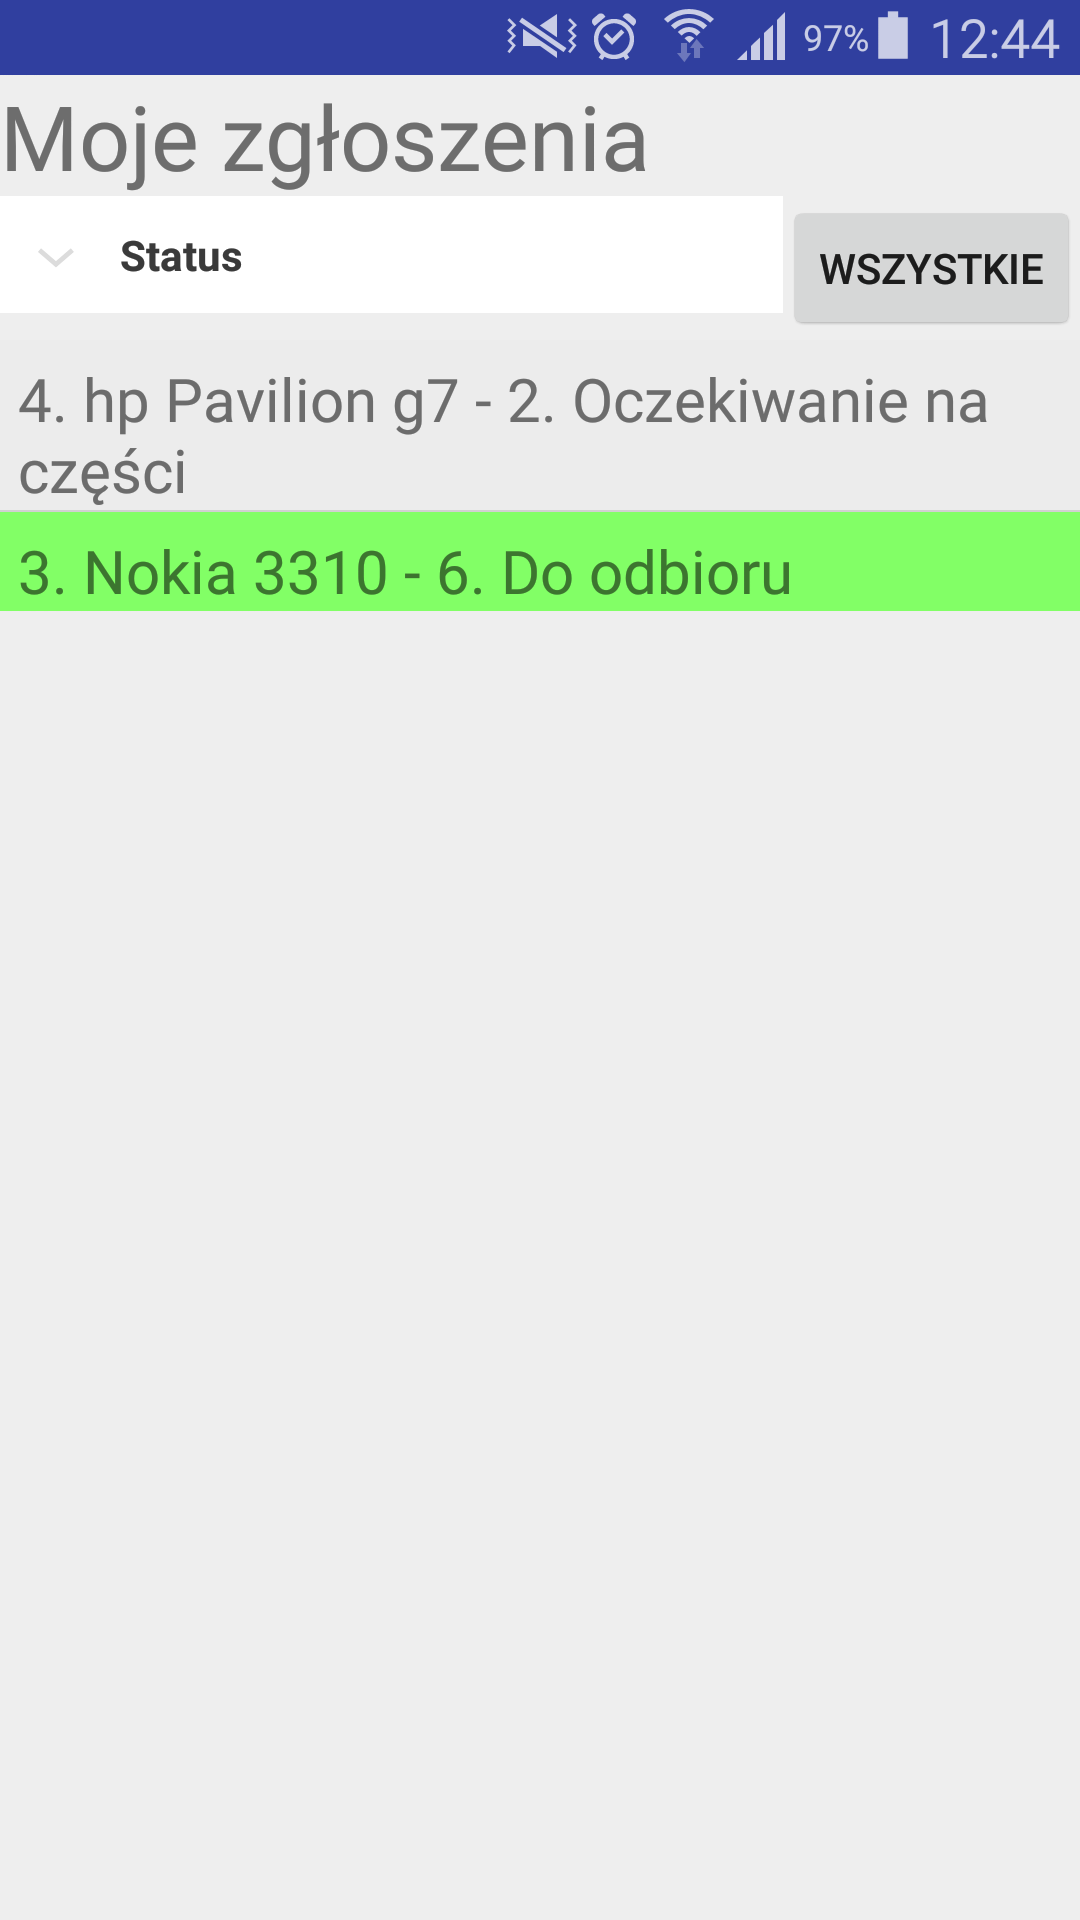
\includegraphics[width=0.6\textwidth,height=0.9\textheight]{zleceniaMobile.png}
	\caption{Zlecenia w~aplikacji mobilnej}
\end{figure}

\begin{figure}[H]
	\centering
	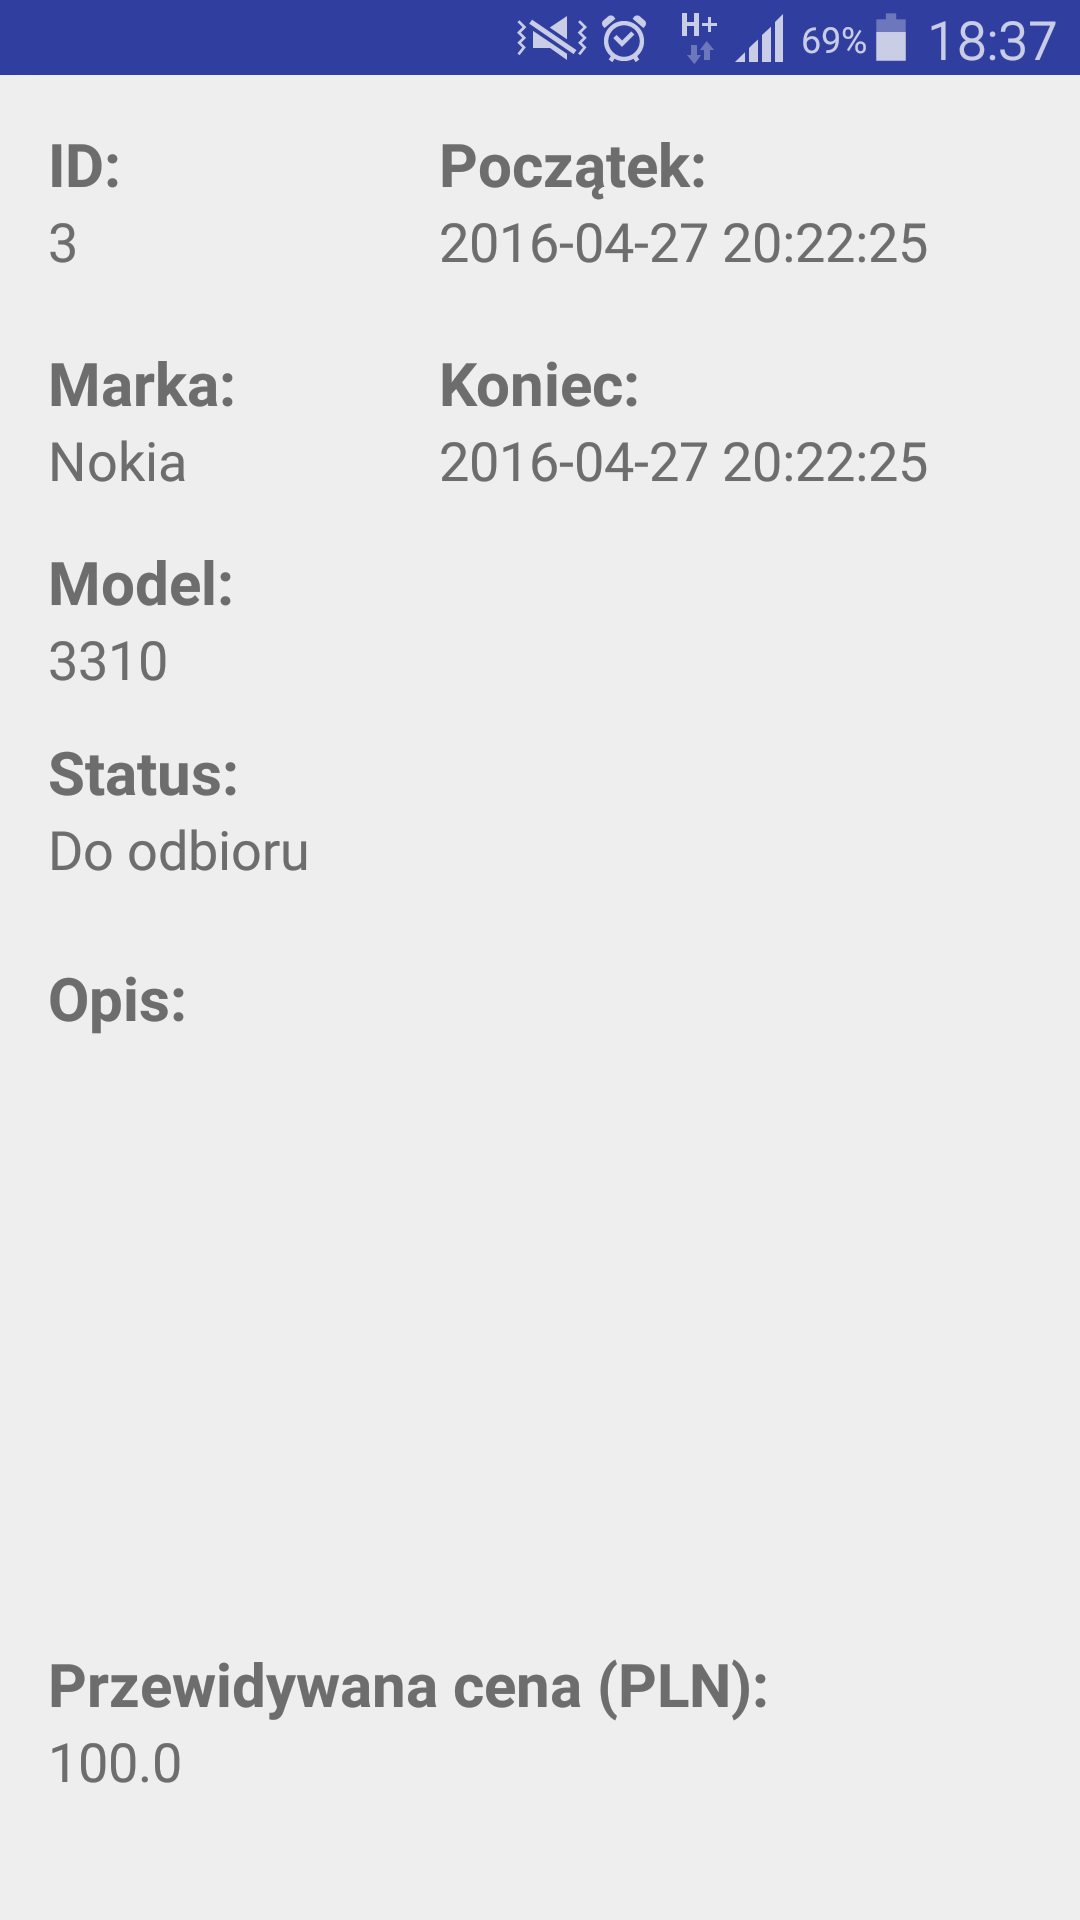
\includegraphics[width=0.6\textwidth,height=0.9\textheight]{szczegolyMobile.png}
	\caption{Szczegóły zlecenia w~aplikacji mobilnej}
\end{figure}





\section{Podsumowanie}
Głównym celem projektu można określić wytworzenie systemu dostępnego zarówno z~poziomu przeglądarki internetowej i~telefonu komórkowego zdolnego do poprawy jakości komunikacji pomiędzy serwisem naprawy wybranych urządzeń a~jego klientem. Patrząc wstecz na ogół zadań wykonanych w~trakcie ostatniego semestru oraz na finalny rezultat poczynionych prac można stwierdzić że nadrzędny cel projektu został bez wątpienia spełniony, a~sam projekt można określić mianem sukcesu.

Dzięki dobrej współpracy wszystkich członków zespołu udało się zrealizować nie tylko wszystkie przewidziane funkcjonalności podstawowe, ale również prawie każdą funkcjonalność rozszerzoną niniejszego projektu. Fakt ten jest tym bardziej godny podziwu, gdyż grupa nigdy wcześniej nie realizowała wspólnie żadnych projektów, a~ponadto część członków dopiero na bieżąco poznawało tajniki technologii wykorzystywanych w~projekcie. Przydatnymi narzędziami okazały się być wykresy Gantta i~platforma Trello, które informowały członków projektu o~aktualnym etapie prac projektowych, ukończonych już fragmentach aplikacji oraz o~ewentualnych opóźnieniach w~realizacji poszczególnych funkcjonalności.

Zrealizowany produkt wyróżnia się na tle innych rozwiązań dostępnych na rynku z~wielu powodów, jednak najbardziej istotne z~nich to otwartość dostarczonego oprogramowania oraz dostarczenie klientowi intuicyjnej aplikacji mobilnej. Podejście takie znacząco upraszcza działania jakie musi wykonać klient aby pozyskać informację z~serwisu napraw, konsekwencją czego jest skrócenie czasu oczekiwania na informacje i~przekłada się na zwiększenie poziomu zadowolenia z~użytkowania aplikacji i~całego projektu. z~tego też względu zachowawczy i~ostrożni, ale jednocześnie pełni optymizmu autorzy są zdania że przy dalszym rozwoju projektu mógłby on stać się de facto standardem w~komunikacji pomiędzy serwisem a~klientem. Taki stan rzeczy z~pewnością przyniósłby poprawę relacji pomiędzy oboma stronami, ocieplił wizerunek serwisów w~oczach klientów oraz pozwolił uniknąć sytuacji takich jak ta, która doprowadziła do powstania koncepcji tego projektu.

\newpage
\listoffigures
\addcontentsline{toc}{section}{Spis rysunków} 
\newpage
\listoftables
\addcontentsline{toc}{section}{Spis tabel}



\newpage
\addcontentsline{toc}{section}{Literatura}
\begin{thebibliography}{9}
\bibitem{cormen} Freedman A., ASP.NET MVC 5 Zaawansowane programowanie, Helion, 2015. 
\bibitem{tabu} JSONObject: https://developer.android.com/reference/org/json/JSONObject.html, dostęp 26.04.2016r.
\bibitem{tabu} Hypertext Transfer Protocol – HTTP/1.1 1999: https://tools.ietf.org/html/rfc2616, dostęp 22.03.2016 r.
\bibitem{bootstrap} Bootstrap 3 Tutorial: http://www.w3schools.com/bootstrap/, dostęp 27.03.2016r.
\bibitem{bootstrap} CSS Tutorial: http://www.w3schools.com/css/, dostęp 04.04.2016r.
\bibitem{jquery} jQuery API: http://api.jquery.com/, dostęp 28.03.2016r.
\end{thebibliography}

\end{document}